% Options for packages loaded elsewhere
\PassOptionsToPackage{unicode}{hyperref}
\PassOptionsToPackage{hyphens}{url}
%
\documentclass[
]{article}
\usepackage{amsmath,amssymb}
\usepackage{iftex}
\ifPDFTeX
  \usepackage[T1]{fontenc}
  \usepackage[utf8]{inputenc}
  \usepackage{textcomp} % provide euro and other symbols
\else % if luatex or xetex
  \usepackage{unicode-math} % this also loads fontspec
  \defaultfontfeatures{Scale=MatchLowercase}
  \defaultfontfeatures[\rmfamily]{Ligatures=TeX,Scale=1}
\fi
\usepackage{lmodern}
\ifPDFTeX\else
  % xetex/luatex font selection
\fi
% Use upquote if available, for straight quotes in verbatim environments
\IfFileExists{upquote.sty}{\usepackage{upquote}}{}
\IfFileExists{microtype.sty}{% use microtype if available
  \usepackage[]{microtype}
  \UseMicrotypeSet[protrusion]{basicmath} % disable protrusion for tt fonts
}{}
\makeatletter
\@ifundefined{KOMAClassName}{% if non-KOMA class
  \IfFileExists{parskip.sty}{%
    \usepackage{parskip}
  }{% else
    \setlength{\parindent}{0pt}
    \setlength{\parskip}{6pt plus 2pt minus 1pt}}
}{% if KOMA class
  \KOMAoptions{parskip=half}}
\makeatother
\usepackage{xcolor}
\usepackage[margin=1in]{geometry}
\usepackage{color}
\usepackage{fancyvrb}
\newcommand{\VerbBar}{|}
\newcommand{\VERB}{\Verb[commandchars=\\\{\}]}
\DefineVerbatimEnvironment{Highlighting}{Verbatim}{commandchars=\\\{\}}
% Add ',fontsize=\small' for more characters per line
\usepackage{framed}
\definecolor{shadecolor}{RGB}{248,248,248}
\newenvironment{Shaded}{\begin{snugshade}}{\end{snugshade}}
\newcommand{\AlertTok}[1]{\textcolor[rgb]{0.94,0.16,0.16}{#1}}
\newcommand{\AnnotationTok}[1]{\textcolor[rgb]{0.56,0.35,0.01}{\textbf{\textit{#1}}}}
\newcommand{\AttributeTok}[1]{\textcolor[rgb]{0.13,0.29,0.53}{#1}}
\newcommand{\BaseNTok}[1]{\textcolor[rgb]{0.00,0.00,0.81}{#1}}
\newcommand{\BuiltInTok}[1]{#1}
\newcommand{\CharTok}[1]{\textcolor[rgb]{0.31,0.60,0.02}{#1}}
\newcommand{\CommentTok}[1]{\textcolor[rgb]{0.56,0.35,0.01}{\textit{#1}}}
\newcommand{\CommentVarTok}[1]{\textcolor[rgb]{0.56,0.35,0.01}{\textbf{\textit{#1}}}}
\newcommand{\ConstantTok}[1]{\textcolor[rgb]{0.56,0.35,0.01}{#1}}
\newcommand{\ControlFlowTok}[1]{\textcolor[rgb]{0.13,0.29,0.53}{\textbf{#1}}}
\newcommand{\DataTypeTok}[1]{\textcolor[rgb]{0.13,0.29,0.53}{#1}}
\newcommand{\DecValTok}[1]{\textcolor[rgb]{0.00,0.00,0.81}{#1}}
\newcommand{\DocumentationTok}[1]{\textcolor[rgb]{0.56,0.35,0.01}{\textbf{\textit{#1}}}}
\newcommand{\ErrorTok}[1]{\textcolor[rgb]{0.64,0.00,0.00}{\textbf{#1}}}
\newcommand{\ExtensionTok}[1]{#1}
\newcommand{\FloatTok}[1]{\textcolor[rgb]{0.00,0.00,0.81}{#1}}
\newcommand{\FunctionTok}[1]{\textcolor[rgb]{0.13,0.29,0.53}{\textbf{#1}}}
\newcommand{\ImportTok}[1]{#1}
\newcommand{\InformationTok}[1]{\textcolor[rgb]{0.56,0.35,0.01}{\textbf{\textit{#1}}}}
\newcommand{\KeywordTok}[1]{\textcolor[rgb]{0.13,0.29,0.53}{\textbf{#1}}}
\newcommand{\NormalTok}[1]{#1}
\newcommand{\OperatorTok}[1]{\textcolor[rgb]{0.81,0.36,0.00}{\textbf{#1}}}
\newcommand{\OtherTok}[1]{\textcolor[rgb]{0.56,0.35,0.01}{#1}}
\newcommand{\PreprocessorTok}[1]{\textcolor[rgb]{0.56,0.35,0.01}{\textit{#1}}}
\newcommand{\RegionMarkerTok}[1]{#1}
\newcommand{\SpecialCharTok}[1]{\textcolor[rgb]{0.81,0.36,0.00}{\textbf{#1}}}
\newcommand{\SpecialStringTok}[1]{\textcolor[rgb]{0.31,0.60,0.02}{#1}}
\newcommand{\StringTok}[1]{\textcolor[rgb]{0.31,0.60,0.02}{#1}}
\newcommand{\VariableTok}[1]{\textcolor[rgb]{0.00,0.00,0.00}{#1}}
\newcommand{\VerbatimStringTok}[1]{\textcolor[rgb]{0.31,0.60,0.02}{#1}}
\newcommand{\WarningTok}[1]{\textcolor[rgb]{0.56,0.35,0.01}{\textbf{\textit{#1}}}}
\usepackage{graphicx}
\makeatletter
\def\maxwidth{\ifdim\Gin@nat@width>\linewidth\linewidth\else\Gin@nat@width\fi}
\def\maxheight{\ifdim\Gin@nat@height>\textheight\textheight\else\Gin@nat@height\fi}
\makeatother
% Scale images if necessary, so that they will not overflow the page
% margins by default, and it is still possible to overwrite the defaults
% using explicit options in \includegraphics[width, height, ...]{}
\setkeys{Gin}{width=\maxwidth,height=\maxheight,keepaspectratio}
% Set default figure placement to htbp
\makeatletter
\def\fps@figure{htbp}
\makeatother
\setlength{\emergencystretch}{3em} % prevent overfull lines
\providecommand{\tightlist}{%
  \setlength{\itemsep}{0pt}\setlength{\parskip}{0pt}}
\setcounter{secnumdepth}{-\maxdimen} % remove section numbering
\ifLuaTeX
  \usepackage{selnolig}  % disable illegal ligatures
\fi
\IfFileExists{bookmark.sty}{\usepackage{bookmark}}{\usepackage{hyperref}}
\IfFileExists{xurl.sty}{\usepackage{xurl}}{} % add URL line breaks if available
\urlstyle{same}
\hypersetup{
  pdftitle={log-project-aubrie-winnie},
  hidelinks,
  pdfcreator={LaTeX via pandoc}}

\title{log-project-aubrie-winnie}
\author{}
\date{\vspace{-2.5em}2024-02-21}

\begin{document}
\maketitle

Understanding how spatial variation is linked to diversity maintenance
in natural communities is a pillar of plant community ecology.
Theoretically, a variable landscape can maintain diversity via niche
partitioning: different species can trade off in performing better or
worse depending on the conditions of the patch they are growing in, and
as a result, more species can sustainably coexist in a community than if
it were spatially heterogeneous. In the hyperdiverse system of native
annual plants in Western Australia, fallen logs may be one of the
greatest contributors to generating spatial variation that could help
maintain species diversity. Considerable anecdotal evidence suggests
that fallen logs generate spatial variation, or patchiness, in the
environment (Figure 1), and that species or assemblages of plants may
respond differently depending on if they are near logs or not. Despite
such anecdotal evidence, it is yet unknown if and how fallen logs
contribute to maintaining species diversity in the native annual plant
communities of the Western Australian wheat belt.

\begin{figure}
\centering
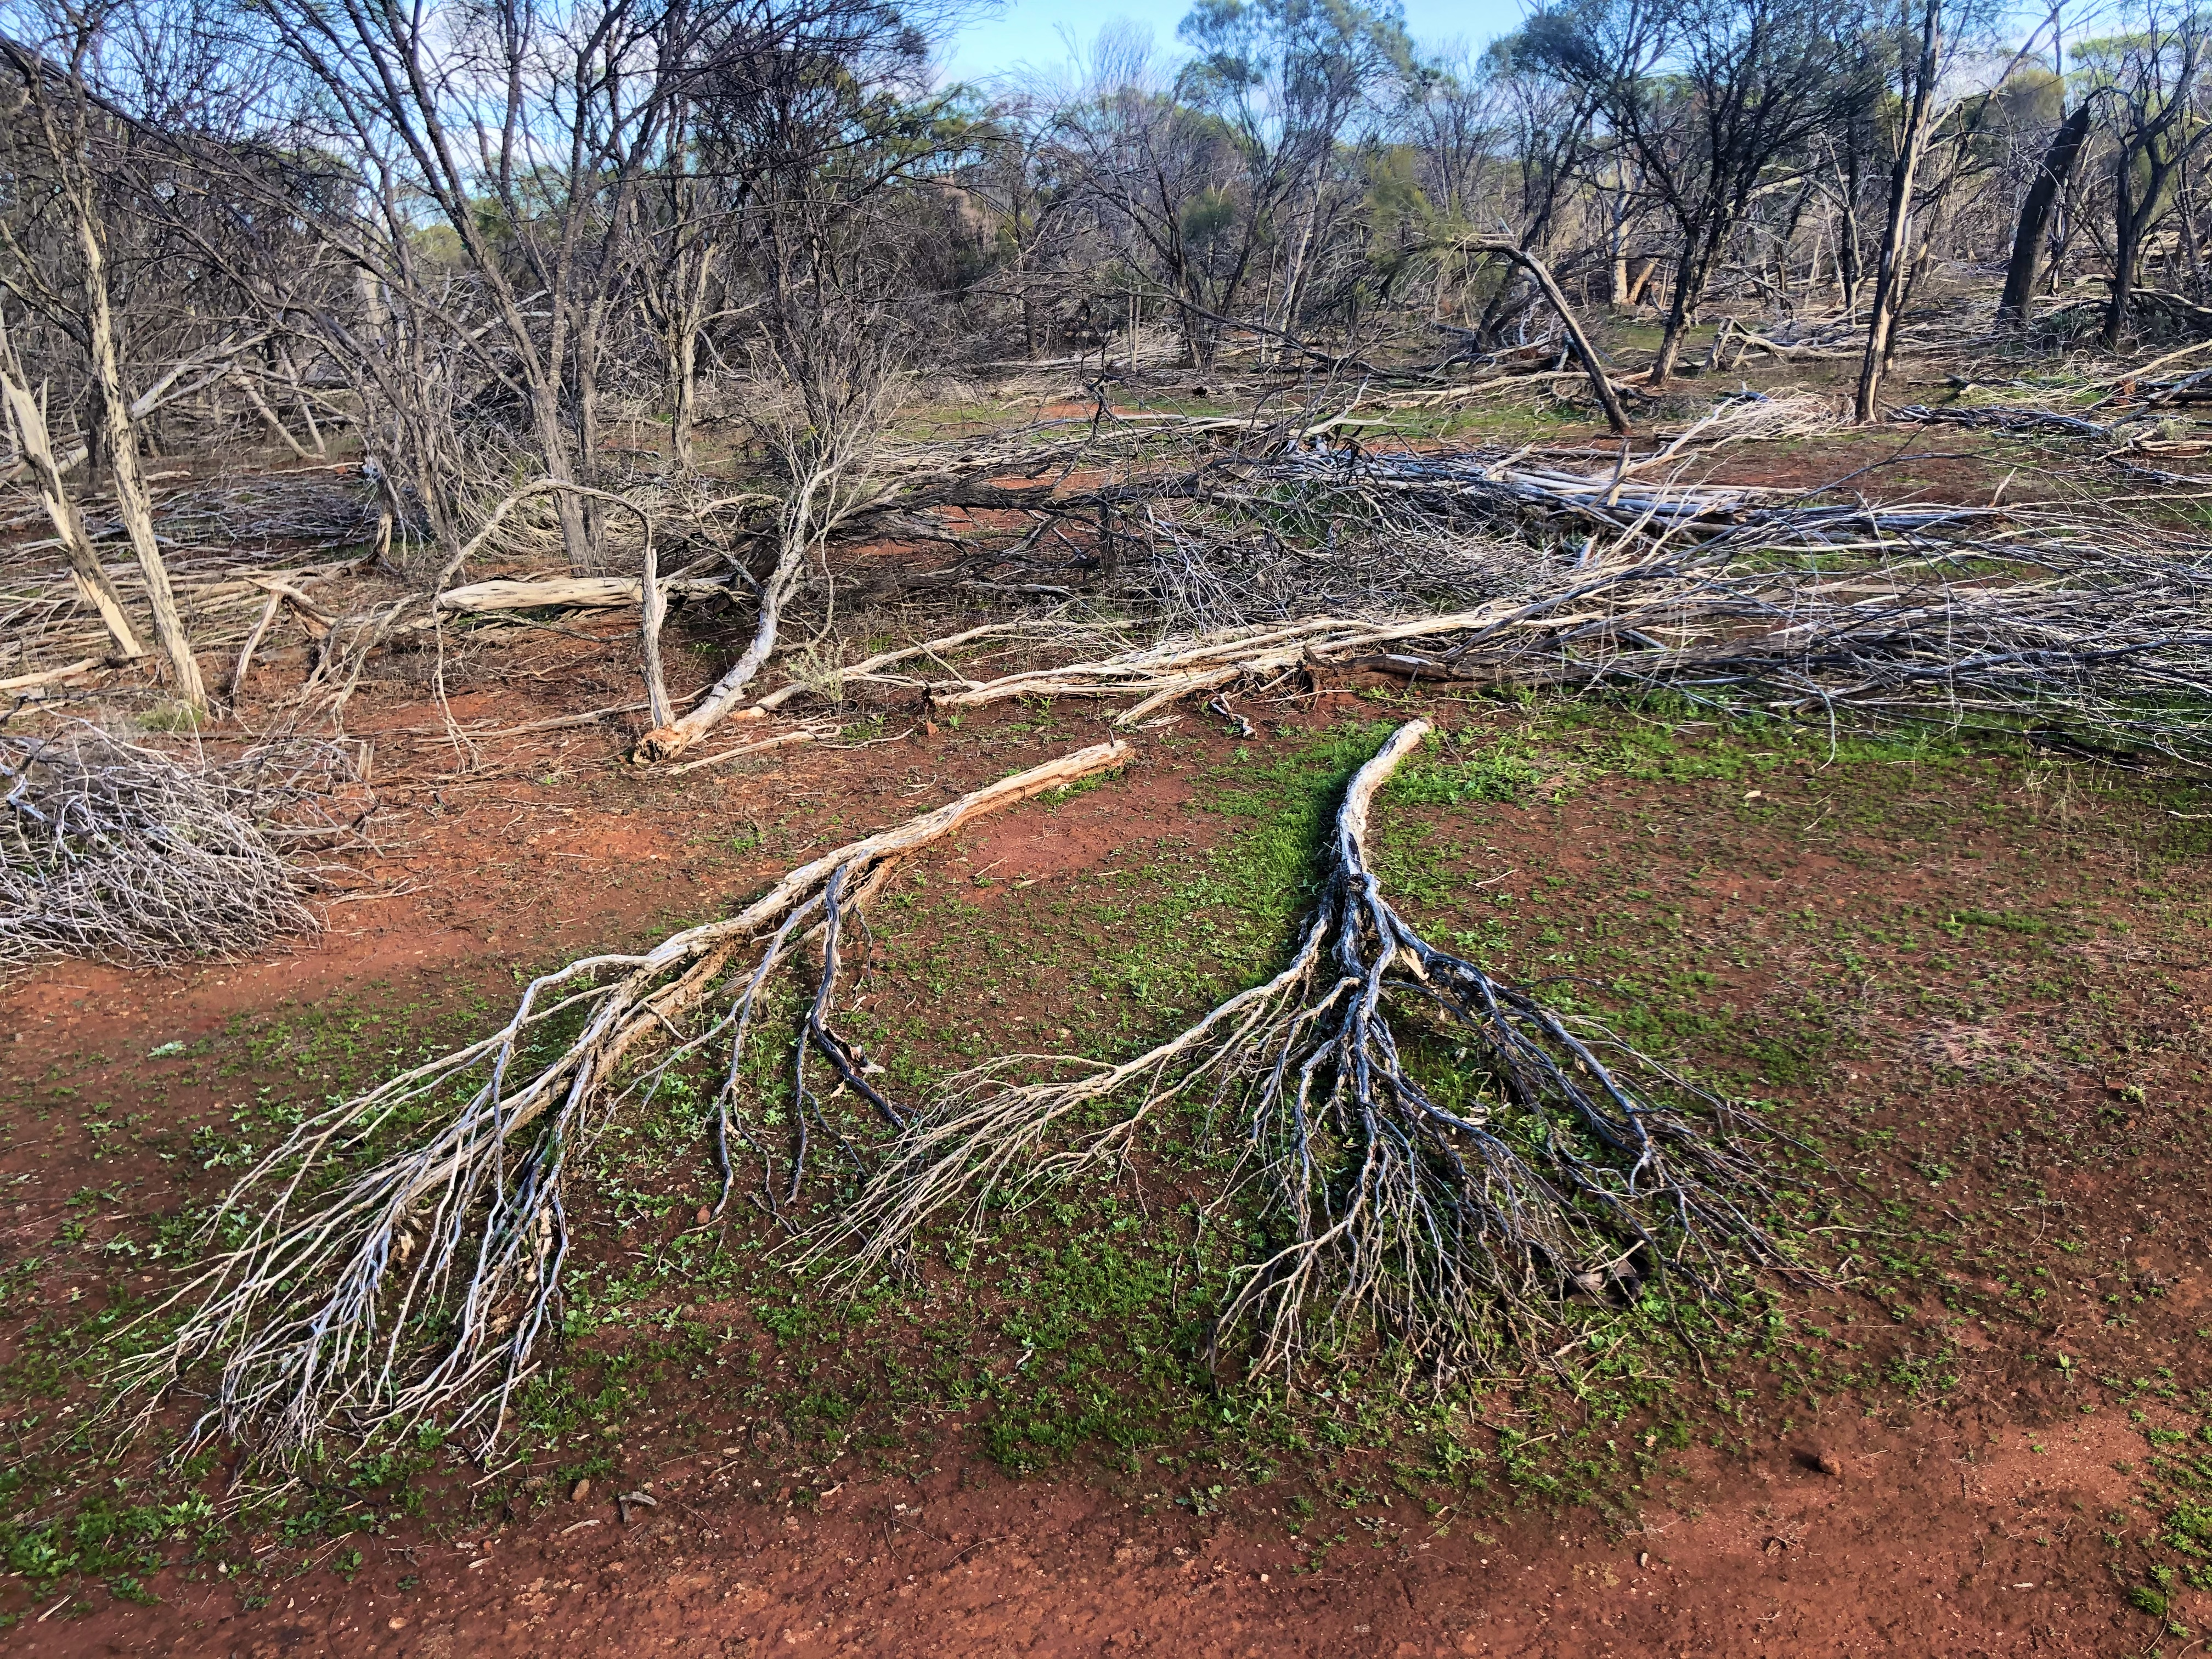
\includegraphics[width=0.5\textwidth,height=\textheight]{example_winter.JPG}
\caption{Figure 1: image of annual plant halos around logs}
\end{figure}

The project will address the following questions:

\textbf{Q1) Are/how are plant communities in fallen log patches
different from patches that are in the open?}

\textbf{Q2) Why are plant communities in fallen log patches different
from patches in the open?}

\textbf{Q3) Are/how are plant species performances affected by proximity
to fallen logs?}

\hypertarget{hypotheses}{%
\subsubsection{Hypotheses}\label{hypotheses}}

The null hypothesis, H0, is that annual plants in fallen log patches are
not different in diversity, abundance, or composition from open patches.

In addition to the null hypothesis, the following constitute four,
non-mutually exclusive hypotheses concerning how fallen logs may
introduce spatial variation in the environment. I include corresponding
predictions for how plant communities may differ between fallen log
patches as compared to open patches. \textbf{H1: Log decomposition
creates islands of fertility directly around the fallen log.} Prediction
1: Nutrient composition around logs will be higher than in open plots

Prediction 2: Variations in nutrient composition in log vs open
environments will correspond to variations in species composition,
abundance, and/or richness in these environments.

Prediction 3: All sown plants will perform best in environments where
organic logs have been left `insitu'. In locations where logs have been
removed or replaced with pvc, the legacy of the nutrient island effect
will yield higher sown plant performance than when compared to locations
where logs have never been. The effect of the nutrient island in
locations where logs have been added to open environments should yeild
higher plant performance over time. \emph{note: performance is measured
in terms of germination rate, survival to fruiting, fecundity, and/or
biomass.}

\textbf{H2: Fallen logs alter the microclimate directly around them by
providing shade.} Prediction 1: Shade and temperature around logs vs in
open plots will be different

Prediction 2: Variation in shade and temperature in log vs open
environments will correspond to variation in species composition,
abundance, and/or richness in these environments.

Prediction 3: All sown plants will perform best in environments where
there are organic or pvc logs, no matter if they have been recently
moved or not.

\textbf{H3: Fallen logs trap dispersing seeds as they are blown along
the ground.}

Prediction 1: Dispersing seeds accumulate around logs, leading to a
denser stand of plants in fallen log patches. Plant abundance in fallen
log patches will be higher as compared to open patches. Rare plants will
be more common in fallen log patches as compared to open patches

Prediction 2: All sown plants will perform the same in all experimental
environments

\textbf{H4: At least some species perform differently according to
variation in log vs.~open environments and have short dispersal kernels,
causing fitness-density covariance}

\begin{figure}
\centering
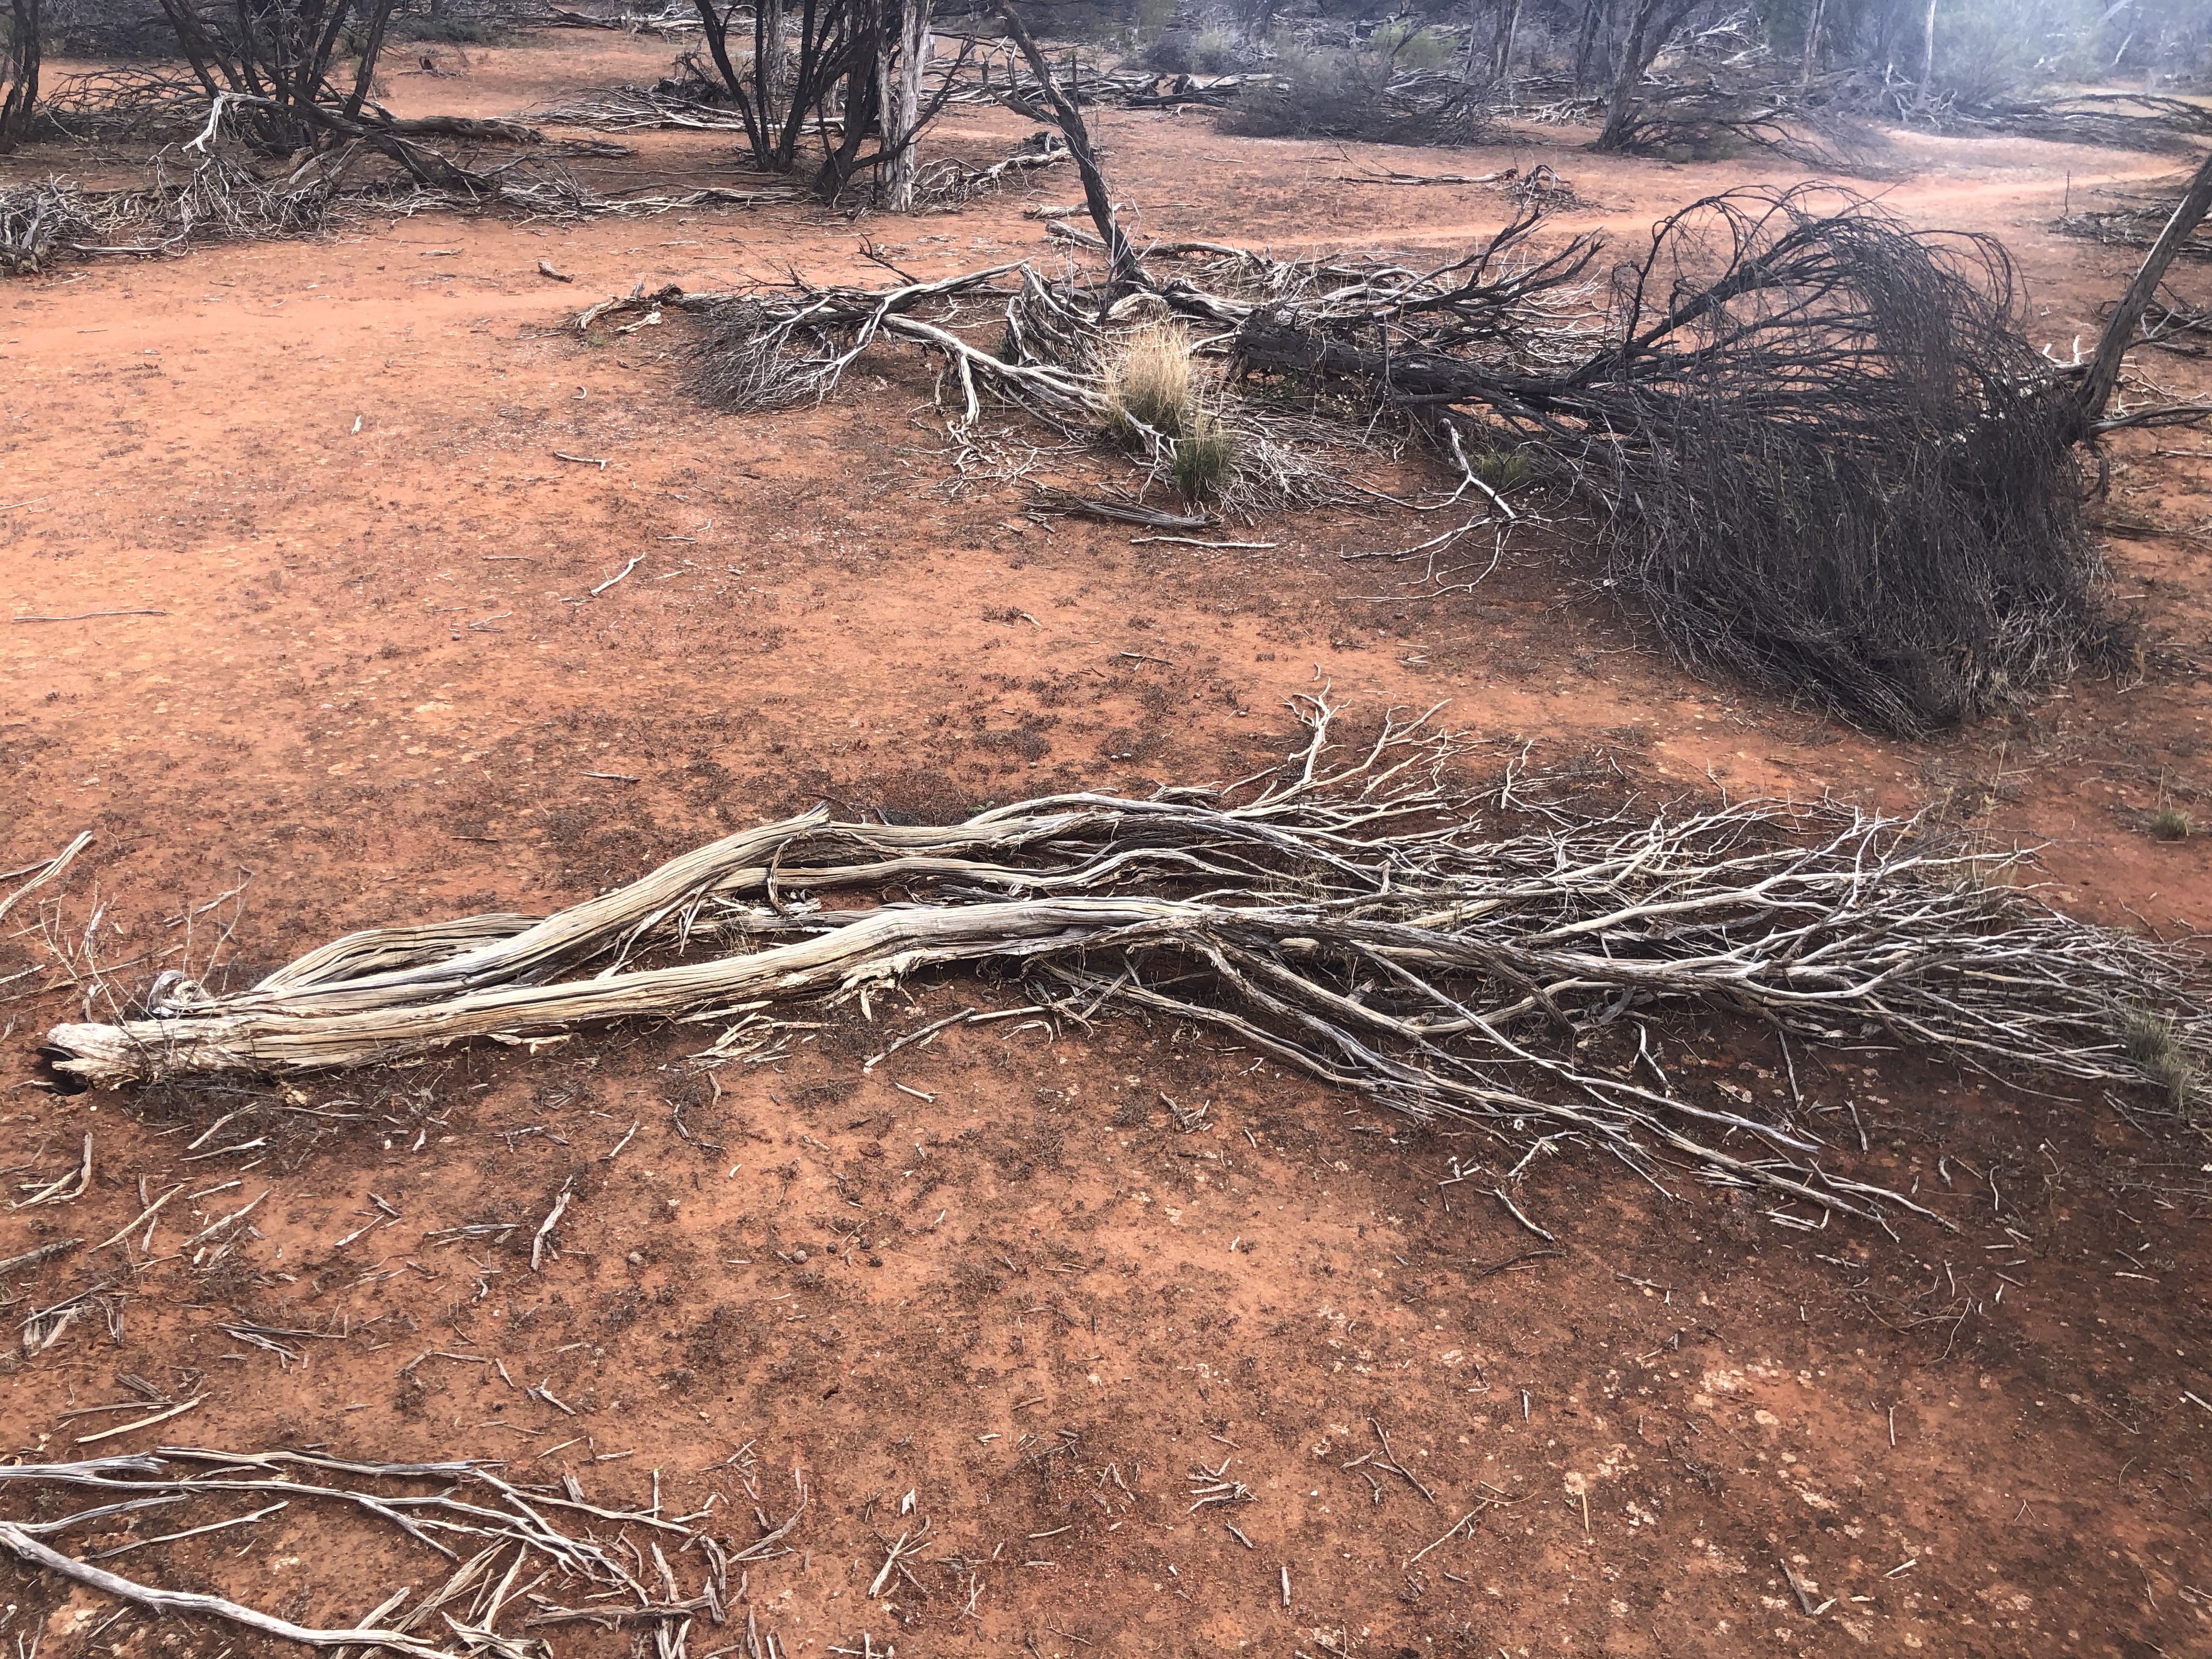
\includegraphics[width=0.5\textwidth,height=\textheight]{wetpatch_example2.jpg}
\caption{Figure 2: Photo before germination, after a rain. Notice the
seeming wet halo under and around the branch}
\end{figure}

\hypertarget{experimental-design}{%
\subsubsection{Experimental Design}\label{experimental-design}}

In this experiment, 224 plots are arranged in 7 blocks of 32 plots each
within the Caron Dam nature reserve.
\href{https://www.google.com/maps/d/edit?mid=1z6w6tScsCcKSpsdUmoupfOJVaaq16VYk\&usp=sharing}{A
map can be found here}. \emph{note: the location info for 3.02 is
probably incorrect as of May 2022, and location info is currently
unavailable for plots 6.25 and 7.19}

Each block is approximately 30m X 30m in area. Plots are 1m long and
linear, and have a pin tag on either end (see Figure 3). The pin tags
have the identity of the plot written on them in the form of
``blocknumber.plotnumber''. Plots are 1m or more away from each other.

In each block, plot environments can be one of six types: - A 1m log
that is out in the open (open\_with\_log, 4 plots) - A 1m log that is a
part of a tree (insitu\_log, 4 plots) - A 1m pvc pipe that is out in the
open (open\_with\_pvc, 4 plots) - A 1m pvc pipe that is a part of a tree
(insitu\_pvc, 4 plots) - A plot that is out in the open (open, 8 plots)
- A gap in a log where a log used to be (gap, 8 plots)

In half of the plots (not including open plots), the addition, exchange,
or removal of logs or pvc to the environment was implemented in October
2020, before seed dispersal. In the other half of these plots, these
manipulations were implemented after seed dispersal, in March 2021.

Within each 1m long plot, there is a \textasciitilde20cm long
microtransect. The ends of the microtransects are marked by a nail and a
washer sunken into the ground. Each microtransect is approximately 21 cm
in internal length from inner washer edge to inner washer edge.
Microtransects are not sided.

In half of all plots, seeds were sown in March 2021 and February 2022.
In these plots, 15 seeds each of Trachymene ornata (TROR), Goodenia
rosea (GORO), and Trachymene cyanopetala (TRCY) are sown outside of the
microtransects as in the diagram. These plants were selected because
they represent plants common to communities next to logs (TROR), out in
the open (GORO), or both (TRCY). The plots where seeds were sown are
called `lambda' plots as noted in Figure 3. In the dataset, the rows
with a ``1'' in the `seeding\_trt' column are the plots that had seeds
sown into them.

\begin{figure}
\centering
\includegraphics[width=0.5\textwidth,height=\textheight]{plottypes2021.png}
\caption{Figure 3: plot schematic}
\end{figure}

\hypertarget{datasets}{%
\subsubsection{Datasets}\label{datasets}}

The sets of data that we have collected for this arm of the project are
the following.

\begin{enumerate}
\def\labelenumi{(\arabic{enumi})}
\tightlist
\item
  Community data, before and after the experiment was implemented.
\end{enumerate}

\begin{itemize}
\tightlist
\item
  Every year during peak biomass we surveyed plant communities at every
  centimeter along each microtransect. Plant count and identity
  information is collected at each centimeter.
\item
  These data are available from 2020 (before the experiment began), 2021
  (one year into the experiment), and 2022 (two years into the
  experiment)
\end{itemize}

\begin{enumerate}
\def\labelenumi{(\arabic{enumi})}
\setcounter{enumi}{1}
\tightlist
\item
  Soil nutrient analysis in the open and insitu log plots.
\end{enumerate}

\begin{itemize}
\tightlist
\item
  In 2022, we sampled 14 samples taken from one insitu\_open plot and
  one insitu\_log plot from each of the seven blocks. At each plot,
  three soil cores from random positions were collected by inserting a
  Hamilton tree planter into a depth of 5 cm. Particularly in
  insitu\_log plots, soil cores were removed within a five-centimeter
  zone adjacent to the wood debris. Between each extraction, all tools
  were sterilised with 80\% ethanol to prevent cross contamination. Soil
  cores from each plot were then mixed, cooled and immediately
  transported to a commercial laboratory (CSBP laboratories). Nutrient
  analysis was conducted at CSBP laboratories to determine soil pH,
  organic C, P, K, inorganic nitrogen (NO3- and NO4+) and basic
  exchangeable cations (Ca, Mg, Na and K). All basic exchangeable
  cations were summed together and labelled as ``CEC''.
\end{itemize}

\begin{enumerate}
\def\labelenumi{(\arabic{enumi})}
\setcounter{enumi}{2}
\tightlist
\item
  Performance data of TROR, TRCY, and TROR.
\end{enumerate}

\begin{itemize}
\item
  In 2021, the only performance data that were collected after sowing
  the experiment were the \textbf{total number of plants that came up
  and survived to fruiting for each species in each location, their
  total biomass, and their per capita biomass}. I calculated per capita
  biomass by dividing total biomass of the collected focal plants by the
  number of focal plants observed. This was because of logistical issues
  due to covid. In this dataset, there were two instances where the
  number of plants collected was greater than the number of seeds sown.
  Both instances were T. cyanopetala, where nplants = 16 and 18. For
  these two datapoints I chose to convert the count values to 15,
  assuming that every individual we planted came up, and that the extra
  were either naturally occurring seeds or that the number of seeds that
  we put into the ground was greater than 15 (human error). To calculate
  total biomass for these two instances, I divided the total biomass by
  the number of individuals observed, and multiplied by 15.
\item
  In 2022, we went to the field early in the season and counted and
  thinned the number of germinated seedlings in each location. We
  therefore have a count for germination, but for the following reasons
  there are some issues with these data. The first is that we probably
  surveyed germination a little too early. The seedlings were often
  super small or hadn't come up yet. Because we couldn't come back later
  to re-thin the plots, we went ahead with counting and thinning
  seedlings. The values in the dataset for 2022
  (nplants\_data\_2022.csv) corresponding to this germination survey are
  ``ntrcy\_germ'', ``ngoro\_germ'' and ``ntror\_germ''. The second is
  that at the end of the growing season, Jake and Winnie came back and
  found that there was often more than one plant of the focal species
  where we seeded them, and sometimes there was one or more focal plants
  that popped up where we had not observed germination earlier in the
  season. We assume that these plants come from the seeds we planted,
  and that they came up later than our initial germination survey. The
  number of plants observed and collected at each location at the end of
  the season are in the columns ``nplants\_tror'', ``nplants\_goro'' and
  ``nplants\_trcy'' in the nplants\_data\_2022.csv data file. Because
  ngerm and nplants don't totally capture what came up where we sowed
  seed, I chose to analyze the total number of observed plants. I
  calculated this as the number of total plants we observed between the
  germination and the end of the season, being careful not to
  double-count the individual that was left after thinning from the
  first round of germination survey. The performance data I analyze here
  are \textbf{total number of plants that came up for each species in
  each location, and the per capita biomass of plants collected at the
  end of the season}.
\end{itemize}

\hypertarget{methods-and-analysis}{%
\subsection{Methods and analysis}\label{methods-and-analysis}}

\hypertarget{q1-arehow-are-plant-communities-in-fallen-log-patches-different-from-patches-that-are-in-the-open}{%
\subsubsection{\texorpdfstring{\textbf{Q1 Are/how are plant communities
in fallen log patches different from patches that are in the open?}
}{Q1 Are/how are plant communities in fallen log patches different from patches that are in the open?  }}\label{q1-arehow-are-plant-communities-in-fallen-log-patches-different-from-patches-that-are-in-the-open}}

\hypertarget{overview-of-results}{%
\paragraph{\texorpdfstring{\emph{Overview of results}
}{Overview of results  }}\label{overview-of-results}}

Quick recap:

\begin{itemize}
\tightlist
\item
  Plant abundance did not differ between log and open patches every
  year.
\item
  Plant diversity is higher in log patches in 2022. When pulling data
  from 2020-2022 together, plant diversity and likelihood of having
  positive Shannon diversity index are higher in log patches.
\item
  Plot type (log vs open) explained a relatively small portion of the
  variance in plant species composition across plots ranging from 6-12\%
  across years. Visually, the composition of plants tends to
  consistently differ between plot types in the non-dimensional space.
\end{itemize}

To compare the characteristic of plant communities in fallen log patches
and open patches, we assessed differences in plant abundance, diversity
using the Shannon diversity index, and plant composition summarized at
the transect level. The analysis is organized by year - we first
analysed plot level community data that was compiled from 2020 to 2022.
In other words, each row in the data set represents an individual plot
from a specific year. After that, we analysed plot level data from 2020,
2021, and 2022 separately. Next, we analysed the plot level data for
each year separately: 2020, 2021, and 2022. This resulted in four levels
of analysis: 1. 2020-2022 composite data, 2. 2020 data, 3. 2021 data,
and 4. 2022 data. For each year, we evaluated three response variables:
abundance, diversity, and plant composition.

\emph{2020-2022} There are three response variables: count (Poisson),
Shannon diversity index (hurdle: binomial and truncated-Gaussian
distributiobns), and composition matrix.

\begin{enumerate}
\def\labelenumi{\arabic{enumi}.}
\tightlist
\item
  \emph{Abundance} -- the abundance of plants in log patches and open
  patches that are similar (treatment: p \textgreater{} 0.05). The
  presented model has a structure of ``count \textasciitilde{}
  treatment(log/open) + (1\textbar block) + (1\textbar year)''.
\item
  \emph{Diversity} -- the probability of having a positive Shannon
  diversity index in the plant community is lower in open patches by
  6.04\% (treatment: p = 0.03). The plant diversity, as measured by the
  Shannon diversity index, is higher in log patches by 0.09 units
  (treatment: p = 0.02). The presented model has a structure of
  ``diversity \textasciitilde{} treatment(log/open) + (1\textbar block)
  + (1\textbar year)''.
\item
  \emph{Composition} -- the five-dimensional NMDS ordination has stress
  values of 9\%, which suggests a fairly good fit for the ordinations.
  Each two-dimensional NMDS plot can be separated into two groups that
  overlap - fallen log patches and open patches. In the nondimensional
  space, the relative position of log plots tend to consistently deviate
  away from open plots. This can be interpreted as a turnover in species
  composition at the scale of the plot type. At the same time, relative
  position of plots sampled from the same block are typically close to
  each other in nondimensional space, reflecting the similarity of plant
  communities at a greater spatial level (i.e.~block).
\end{enumerate}

Adjusted R2 of the partial RDA is 5.62\%. The conditioned terms Block
and Year accounted for 44.3\% of variations in species composition. Plot
type (constrained term) accounted for about 6\% of variations in species
composition. 49.6\% of variation is unexplained (unconstrained).

\emph{2020}

There are three response variables: count (Poisson), Shannon diversity
index (hurdle: binomial and Gaussian), and composition matrix.

\begin{enumerate}
\def\labelenumi{\arabic{enumi}.}
\tightlist
\item
  \emph{Abundance} -- the abundance of plants in log patches and open
  patches that are similar (treatment: p \textgreater{} 0.05). The
  presented model has a structure of ``count \textasciitilde{}
  treatment(log/open) + (1\textbar block)''.
\item
  \emph{Diversity} -- the plant diversity and the probability of having
  a positive Shannon diversity index in the plant community between log
  and open patches are similar (treatment: p \textgreater{} 0.05). The
  presented model has a structure of ``diversity \textasciitilde{}
  treatment(log/open) + (1\textbar block)''.
\item
  \emph{Composition} -- the four-dimensional NMDS ordination has stress
  values of 4.8\%, which suggests a very good fit for the ordinations.
  Similar discussion as in \emph{2020-2022}.
\end{enumerate}

Adjusted R2 of the partial RDA is 8.5\%. The conditioned term, Block,
accounted for 69.6\% of variations in species composition. Plot type
(constrained term) accounted for about 8.3\% of variations in species
composition. 22.6\% of variation is unexplained (unconstrained).

\emph{2021}

There are three response variables: count (Poisson), Shannon diversity
index (hurdle: binomial and Gaussian), and composition matrix.

\begin{enumerate}
\def\labelenumi{\arabic{enumi}.}
\tightlist
\item
  \emph{Abundance} -- the abundance of plants in log patches and open
  patches that are similar (treatment: p \textgreater{} 0.05). The
  presented model has a structure of ``count \textasciitilde{}
  treatment(log/open) + (1\textbar block)''.
\item
  \emph{Diversity} -- the plant diversity and the probability of having
  a positive Shannon diversity index in the plant community between log
  and open patches are similar (treatment: p \textgreater{} 0.05). The
  presented model has a structure of ``diversity \textasciitilde{}
  treatment(log/open) + (1\textbar block)''.
\item
  \emph{Composition} -- The five-dimensional NMDS ordination has stress
  values of 4.1\%, which suggests a very good fit for the ordinations.
  Similar discussion as in \emph{2020-2022}.
\end{enumerate}

Adjusted R2 of the partial RDA is 11.9\%. The conditioned term, Block,
accounted for 53.7\% of variations in species composition. Plot type
(constrained term) accounted for about 12.1\% of variations in species
composition. 34.2\% of variation is unexplained (unconstrained).

\emph{2022}

There are three response variables: count (Poisson), Shannon diversity
index (hurdle: binomial and Gaussian), and composition matrix.

\begin{enumerate}
\def\labelenumi{\arabic{enumi}.}
\tightlist
\item
  \emph{Abundance} -- the abundance of plants in log patches and open
  patches that are similar (treatment: p \textgreater{} 0.05). The
  presented model has a structure of ``count \textasciitilde{}
  treatment(log/open) + (1\textbar block)''.
\item
  \emph{Diversity} -- the probability of having a positive Shannon
  diversity index in the plant community between log and open patches
  are similar (treatment: p \textgreater{} 0.05). The plant diversity,
  as measured by the Shannon diversity index, higher in log patches by
  0.24 units (treatment: p = 0.007). The presented model has a structure
  of ``diversity \textasciitilde{} treatment(log/open) +
  (1\textbar block)''.
\item
  \emph{Composition} -- The five-dimensional NMDS ordination has stress
  values of 4\%, which suggests a very good fit for the ordinations.
  Similar discussion as in \emph{2020-2022}.
\end{enumerate}

Adjusted R2 of the partial RDA is 11.0\%. The conditioned term, Block,
accounted for 55.7\% of variations in species composition. Plot type
(constrained term) accounted for about 11.4\% of variations in species
composition. 33.0\% of variation is unexplained (unconstrained).

\hypertarget{statistical-methods}{%
\paragraph{\texorpdfstring{\emph{Statistical Methods}
}{Statistical Methods  }}\label{statistical-methods}}

\begin{enumerate}
\def\labelenumi{\arabic{enumi}.}
\tightlist
\item
  Abundance comparison
\end{enumerate}

Comparison of plant abundance between log patches and open patches
involves two types of data: (1) plant counts of all plots in 2020 before
the experiment setup differentiated by the initial treatment ``log'' and
``open''; and (2) plant counts from insitu\_log and insitu\_open plots
in 2021 and 2022 respectively. All count data used for abundance
comparison includes species with unknown identity. We used a generalized
linear mixed-effects model (GLMER) to model the abundance of plant
individuals (2020, 2021 and 2022 data) in unaltered fallen log patches
and open patches using a Poisson distribution structure with block as
random terms. When pulling count data from 2020 to 2022 together, we
included time as a random term to avoid pseudo-replication.

\begin{enumerate}
\def\labelenumi{\arabic{enumi}.}
\setcounter{enumi}{1}
\tightlist
\item
  Diversity comparison
\end{enumerate}

A 20-centimeter linear transect was set up for each plot in 2020. We
recorded species identity and individual counts for all species
occurring along the transects in 2020, 2021 and 2022 respectively.
Comparison of plant diversity between log patches and open patches
involves two types of data: (1) plant count for each species of all
plots in 2020 before the experiment setup differentiated by the initial
treatment ``log'' and ``open''; and (2) plant count for each species
from insitu\_log and insitu\_open plots in 2021 and 2022 respectively.
All data used for diversity comparison excludes species with unknown
identity.

We used the Shannon diversity index to calculate the plant species
diversity for each transect at the plot level. A considerable number of
zeros are generated in the computation of the Shannon diversity index.
We first tried modelling diversity data with a linear mixed-effect model
(LMER) assuming a Gaussian distribution. The resulting model was
zero-inflated as testing with DHARMa.

As a solution, we used a two-component hurdle model on the truncated
data set where the response diversity index was separated into zero and
non-zero values. In the first component, we used a binomial GLMER to
model the probability of zeros and non-zeros in the diversity index with
blocks as random terms. For the second component, we assumed an
approximate Gaussian distribution of the non-zero Shannon index and used
a linear mixed-effects regression (LMER) to model the response non-zero
diversity index with treatment as a fixed effect (log vs open) and block
as a random factor. Specifically, for the hurdle model on composite
diversity data (2020 to 2022), we also included year as a random factor.

\begin{enumerate}
\def\labelenumi{\arabic{enumi}.}
\setcounter{enumi}{2}
\tightlist
\item
  Composition
\end{enumerate}

Comparison of plant composition between log patches and open patches
involves two types of data: (1) plant count for each species of all
plots in 2020 before the experiment setup differentiated by the initial
treatment ``log'' and ``open''; and (2) plant count for each species
from insitu\_log and insitu\_open plots in 2021 and 2022 respectively.
All data used for diversity comparison excludes species with unknown
identity. For transects where no plants were found, an artificial
species, ``x,'' was added to the species composition matrix to represent
zero plants.

We used Non-Metric Dimensional Scaling (NMDS) to analyse the differences
in plant communities with Bray-Curtis dissimilarity metrics. We retained
two dimensions in the NMDS ordination plot for the visualization and
interpretation of plant community composition differences between plot
types and blocks.

To identify the contribution of each species to the compositional
changes amongst different sample plots, we extracted ordination scores
for each species along NMDS axes 1 and 2. The species scores represent
the weighted average of a species' abundance score in a sample community
along our selected NMDS axes. We also ran a partial Redundancy Analysis
(RDA) to test the correlation between species composition (squared-root
transformed) and plot type (log vs open patch) with block as a random
term.

\hypertarget{analysis}{%
\paragraph{\texorpdfstring{\emph{Analysis}}{Analysis }}\label{analysis}}

\hypertarget{abundance-analysis}{%
\subparagraph{Abundance analysis}\label{abundance-analysis}}

** 2020 - 2022 **

~

Abundance:2020-2022

Abundance:2020

Abundance:2021

Abundance:2022

Predictors

Incidence Rate Ratios

CI

p

Incidence Rate Ratios

CI

p

Incidence Rate Ratios

CI

p

Incidence Rate Ratios

CI

p

(Intercept)

6.79

4.88~--~9.46

\textless0.001

4.74

4.34~--~5.18

\textless0.001

7.14

6.20~--~8.22

\textless0.001

8.82

7.56~--~10.30

\textless0.001

init {[}open{]}

1.00

0.93~--~1.09

0.913

0.94

0.83~--~1.07

0.355

1.09

0.92~--~1.28

0.322

1.04

0.89~--~1.21

0.642

Random Effects

σ2

0.14

0.20

0.12

0.10

τ00

0.00 block

0.00 block

0.00 block

0.01 block

0.08 time

~

~

~

ICC

0.38

0.00

0.03

0.12

N

7 block

7 block

7 block

7 block

3 time

~

~

~

Observations

391

221

86

84

Marginal R2 / Conditional R2

0.000 / 0.378

0.004 / 0.009

0.012 / 0.037

0.002 / 0.127

\includegraphics{log-project-aubrie-winnie_files/figure-latex/unnamed-chunk-1-1.pdf}
\includegraphics{log-project-aubrie-winnie_files/figure-latex/unnamed-chunk-1-2.pdf}

\hypertarget{diversity-analysis}{%
\subparagraph{Diversity analysis}\label{diversity-analysis}}

\begin{verbatim}
## Loading required package: lmerTest
\end{verbatim}

\begin{verbatim}
## 
## Attaching package: 'lmerTest'
\end{verbatim}

\begin{verbatim}
## The following object is masked from 'package:lme4':
## 
##     lmer
\end{verbatim}

\begin{verbatim}
## The following object is masked from 'package:stats':
## 
##     step
\end{verbatim}

\begin{verbatim}
## Loading required package: performance
\end{verbatim}

\begin{verbatim}
## Loading required package: DHARMa
\end{verbatim}

\begin{verbatim}
## This is DHARMa 0.4.6. For overview type '?DHARMa'. For recent changes, type news(package = 'DHARMa')
\end{verbatim}

\begin{verbatim}
## Loading required package: patchwork
\end{verbatim}

\begin{verbatim}
## Warning in labdsv::matrify(commsub): NAs introduced by coercion
\end{verbatim}

\begin{verbatim}
## `summarise()` has grouped output by 'time', 'block', 'transect', 'init'. You
## can override using the `.groups` argument.
\end{verbatim}

Shannon diversity index (SDI): 2020-2022

~

Prob. SDI\textgreater0

Pron. when SDI\textgreater0

Predictors

Log-Odds

std. Error

CI

p

Estimates

std. Error

CI

p

(Intercept)

2.24

0.47

1.32~--~3.17

\textless0.001

1.08

0.05

0.98~--~1.17

\textless0.001

init {[}open{]}

-0.60

0.28

-1.15~--~-0.06

0.030

-0.09

0.04

-0.17~--~-0.02

0.019

Random Effects

σ2

3.29

0.12

τ00

0.12 block

0.00 block

0.40 time

0.00 time

ICC

0.13

0.04

N

7 block

7 block

3 time

3 time

Observations

393

319

Marginal R2 / Conditional R2

0.023 / 0.155

0.017 / 0.059

Shannon diversity index (SDI): 2020

~

Prob. SDI\textgreater0

Pron. when SDI\textgreater0

Predictors

Log-Odds

std. Error

CI

p

Estimates

std. Error

CI

p

(Intercept)

1.25

0.25

0.76~--~1.74

\textless0.001

1.00

0.04

0.93~--~1.08

\textless0.001

init {[}open{]}

-0.37

0.31

-0.97~--~0.24

0.235

-0.08

0.05

-0.19~--~0.02

0.132

Random Effects

σ2

3.29

~

τ00

0.06 block

~

ICC

0.02

~

N

7 block

~

Observations

223

165

Marginal R2 / Conditional R2

0.010 / 0.029

0.014 / 0.008

Shannon diversity index (SDI): 2021

~

Prob. SDI\textgreater0

Pron. when SDI\textgreater0

Predictors

Log-Odds

std. Error

CI

p

Estimates

std. Error

CI

p

(Intercept)

3.37

1.02

1.83~--~6.25

0.001

1.06

0.06

0.93~--~1.19

\textless0.001

init {[}open{]}

-1.42

1.09

-4.38~--~0.37

0.194

0.00

0.08

-0.16~--~0.16

0.981

Random Effects

σ2

~

0.11

τ00

~

0.00 block

ICC

~

0.02

N

~

7 block

Observations

86

78

R2 Tjur

0.023

0.000 / 0.017

\begin{verbatim}
## Warning in checkConv(attr(opt, "derivs"), opt$par, ctrl = control$checkConv, : Model is nearly unidentifiable: large eigenvalue ratio
##  - Rescale variables?
\end{verbatim}

Shannon diversity index (SDI): 2022

~

Prob. SDI\textgreater0

Pron. when SDI\textgreater0

Predictors

Log-Odds

std. Error

CI

p

Estimates

std. Error

CI

p

(Intercept)

29.87

547.35

-1042.92~--~1102.66

0.956

1.21

0.08

1.06~--~1.36

\textless0.001

init {[}open{]}

-27.70

547.35

-1100.48~--~1045.09

0.960

-0.24

0.09

-0.41~--~-0.07

0.007

Random Effects

σ2

3.29

0.13

τ00

1.15 block

0.01 block

ICC

0.26

0.07

N

7 block

7 block

Observations

84

76

Marginal R2 / Conditional R2

0.975 / 0.981

0.088 / 0.149

\includegraphics{log-project-aubrie-winnie_files/figure-latex/unnamed-chunk-2-1.pdf}

\hypertarget{composition-analysis}{%
\subparagraph{Composition analysis}\label{composition-analysis}}

Composition dissimilarity * 2020 *

\includegraphics{log-project-aubrie-winnie_files/figure-latex/unnamed-chunk-5-1.pdf}

\begin{verbatim}
## 
## Call:
## rda(X = ass.rel.t0, Y = init, Z = block) 
## 
## Partitioning of variance:
##               Inertia Proportion
## Total         0.42624    1.00000
## Conditioned   0.29429    0.69045
## Constrained   0.03551    0.08332
## Unconstrained 0.09643    0.22624
## 
## Eigenvalues, and their contribution to the variance 
## after removing the contribution of conditiniong variables
## 
## Importance of components:
##                          RDA1     PC1     PC2     PC3     PC4     PC5      PC6
## Eigenvalue            0.03551 0.03207 0.02047 0.01524 0.01394 0.01034 0.004375
## Proportion Explained  0.26916 0.24303 0.15511 0.11552 0.10566 0.07837 0.033159
## Cumulative Proportion 0.26916 0.51219 0.66730 0.78282 0.88848 0.96684 1.000000
## 
## Accumulated constrained eigenvalues
## Importance of components:
##                          RDA1
## Eigenvalue            0.03551
## Proportion Explained  1.00000
## Cumulative Proportion 1.00000
## 
## Scaling 2 for species and site scores
## * Species are scaled proportional to eigenvalues
## * Sites are unscaled: weighted dispersion equal on all dimensions
## * General scaling constant of scores:  1.534259 
## 
## 
## Species scores
## 
##             RDA1        PC1        PC2        PC3        PC4        PC5
## acul   0.1067309 -9.564e-02 -2.516e-02  6.791e-02 -5.735e-02 -1.985e-02
## aicu   0.0342552  7.579e-02 -2.904e-02 -1.040e-01 -1.656e-02  3.629e-04
## arca   0.0000000 -1.038e-17 -5.555e-18 -3.808e-18 -5.876e-18 -1.336e-18
## ardy   0.0000000  3.111e-17  1.887e-17 -2.100e-17 -3.214e-17 -4.399e-18
## arsp   0.0212814 -9.296e-03  3.074e-02 -1.243e-02  2.902e-02  2.380e-02
## auel   0.0000000  1.554e-17  1.431e-17  2.485e-18  1.338e-17  1.717e-18
## bldr   0.0627812 -3.489e-02  5.885e-02 -3.487e-02  5.598e-02 -1.193e-01
## blrd   0.0000000 -1.043e-17 -2.030e-18 -1.775e-18  5.772e-18  4.877e-18
## brdi   0.0000000 -3.310e-18 -1.477e-17  8.060e-18 -1.579e-18 -7.770e-18
## brdr   0.0000000 -2.281e-17  3.884e-18  9.274e-18  4.319e-17  1.140e-17
## brpe   0.0000000  6.077e-18 -2.852e-18 -1.460e-18 -1.222e-17 -4.230e-18
## brru   0.0000000  2.866e-32  1.924e-32 -2.506e-32 -4.481e-32  1.525e-33
## buse  -0.0399181  8.064e-03 -8.920e-03 -7.638e-03 -1.217e-02  6.087e-02
## caer  -0.0770469  5.739e-03 -4.007e-02  2.232e-02 -3.681e-02  4.977e-02
## cagr  -0.0353354  3.492e-02 -5.082e-02 -7.084e-02  2.218e-02  4.523e-02
## cahi   0.0073560  1.491e-02  4.828e-02 -6.274e-03  3.863e-02  1.972e-02
## casp   0.0071091 -7.320e-02 -4.968e-02  8.494e-03  2.080e-02  8.123e-03
## cear   0.0000000  0.000e+00  0.000e+00  0.000e+00  0.000e+00  0.000e+00
## chau   0.0270050  2.642e-02  5.365e-02 -7.004e-02 -9.242e-02 -2.682e-03
## chei   0.0000000  0.000e+00  0.000e+00  0.000e+00  0.000e+00  0.000e+00
## chps   0.0867979 -8.706e-02 -4.807e-02  5.256e-03 -3.053e-02 -5.813e-02
## crcl   0.0000000  0.000e+00  0.000e+00  0.000e+00  0.000e+00  0.000e+00
## crco  -0.0054567 -2.817e-02 -2.789e-02 -6.578e-02 -6.492e-03  6.700e-02
## cusc   0.0000000  0.000e+00  0.000e+00  0.000e+00  0.000e+00  0.000e+00
## cusp   0.0000000  0.000e+00  0.000e+00  0.000e+00  0.000e+00  0.000e+00
## dagl  -0.0005158 -4.170e-02 -1.197e-02  1.578e-02 -3.486e-02  3.748e-02
## dosp   0.0000000  0.000e+00  0.000e+00  0.000e+00  0.000e+00  0.000e+00
## ento   0.0000000  0.000e+00  0.000e+00  0.000e+00  0.000e+00  0.000e+00
## erau   0.0000000  0.000e+00  0.000e+00  0.000e+00  0.000e+00  0.000e+00
## ercy   0.0000000  0.000e+00  0.000e+00  0.000e+00  0.000e+00  0.000e+00
## erra  -0.0017634  1.363e-03 -1.961e-03 -2.641e-03  6.378e-04  2.340e-03
## ersp  -0.0209707  1.621e-02 -2.332e-02 -3.140e-02  7.584e-03  2.783e-02
## gite  -0.0057450 -7.634e-03  5.428e-03 -7.119e-03 -3.080e-03 -1.608e-03
## gnte   0.0000000  0.000e+00  0.000e+00  0.000e+00  0.000e+00  0.000e+00
## gobe  -0.0320039 -3.133e-03 -9.076e-02  5.077e-02  1.243e-01  2.247e-02
## gocy  -0.0012808  6.463e-02  4.761e-02 -1.112e-02 -1.947e-02 -4.368e-03
## gono   0.0000000  0.000e+00  0.000e+00  0.000e+00  0.000e+00  0.000e+00
## goro   0.0215820  2.211e-01 -1.082e-01 -1.141e-02 -4.094e-02 -1.836e-02
## gosp   0.0446889  2.138e-02  1.224e-02  1.185e-02  3.669e-02  2.988e-02
## haod  -0.0050284 -3.182e-02  7.735e-03  1.165e-02  6.116e-02  1.742e-02
## hygl   0.0601486  6.535e-02  7.287e-02  6.640e-02 -5.544e-02  7.196e-02
## hypi   0.0000000  0.000e+00  0.000e+00  0.000e+00  0.000e+00  0.000e+00
## hypo   0.0000000  0.000e+00  0.000e+00  0.000e+00  0.000e+00  0.000e+00
## jubu   0.0000000  0.000e+00  0.000e+00  0.000e+00  0.000e+00  0.000e+00
## laro  -0.1146604 -4.765e-02 -1.202e-02  3.910e-02 -4.021e-02 -1.545e-02
## ledu   0.0000000  0.000e+00  0.000e+00  0.000e+00  0.000e+00  0.000e+00
## lele   0.0212814 -9.296e-03  3.074e-02 -1.243e-02  2.902e-02  2.380e-02
## loef   0.0000000  0.000e+00  0.000e+00  0.000e+00  0.000e+00  0.000e+00
## misp  -0.0859180  4.494e-02 -1.140e-01 -3.971e-02 -2.276e-02  5.166e-03
## mite   0.0000000  0.000e+00  0.000e+00  0.000e+00  0.000e+00  0.000e+00
## momo   0.0000000  0.000e+00  0.000e+00  0.000e+00  0.000e+00  0.000e+00
## mopa   0.0000000  0.000e+00  0.000e+00  0.000e+00  0.000e+00  0.000e+00
## niro   0.0000000  0.000e+00  0.000e+00  0.000e+00  0.000e+00  0.000e+00
## omco   0.0102406 -1.780e-02 -1.290e-02 -4.528e-03 -7.063e-03  3.001e-03
## orsp   0.0000000  0.000e+00  0.000e+00  0.000e+00  0.000e+00  0.000e+00
## pala   0.0212814 -9.296e-03  3.074e-02 -1.243e-02  2.902e-02  2.380e-02
## peai   0.0697049  5.909e-02 -2.821e-03  5.278e-02 -3.971e-02 -2.331e-02
## pedu   0.0300964 -1.315e-02  4.347e-02 -1.758e-02  4.104e-02  3.366e-02
## phsu   0.0000000  0.000e+00  0.000e+00  0.000e+00  0.000e+00  0.000e+00
## plde   0.0000000  0.000e+00  0.000e+00  0.000e+00  0.000e+00  0.000e+00
## poar   0.0000000  0.000e+00  0.000e+00  0.000e+00  0.000e+00  0.000e+00
## poca   0.0311535  7.429e-02  1.806e-02  8.779e-02  2.715e-02 -2.008e-02
## pocap  0.0157620  1.774e-02  1.191e-02 -1.551e-02 -2.774e-02  9.443e-04
## poce   0.0000000  0.000e+00  0.000e+00  0.000e+00  0.000e+00  0.000e+00
## pogn   0.0000000  0.000e+00  0.000e+00  0.000e+00  0.000e+00  0.000e+00
## pole  -0.0067798  6.543e-02  2.974e-02  8.404e-02 -4.950e-03 -2.006e-02
## pomu   0.1806915 -8.052e-02 -1.066e-01  1.495e-02 -1.385e-02 -5.198e-02
## pter   0.0000000  0.000e+00  0.000e+00  0.000e+00  0.000e+00  0.000e+00
## ptga  -0.0265218  3.413e-02  8.198e-05  2.118e-02  4.241e-02  3.353e-02
## ptob   0.0000000  0.000e+00  0.000e+00  0.000e+00  0.000e+00  0.000e+00
## rhla   0.0114587  1.612e-02 -1.907e-02  1.253e-01 -6.133e-02  3.825e-02
## rhpy  -0.0614885  1.909e-01  1.451e-02  3.551e-03  8.057e-02 -4.550e-02
## rhsp   0.0000000  0.000e+00  0.000e+00  0.000e+00  0.000e+00  0.000e+00
## ry     0.0000000  0.000e+00  0.000e+00  0.000e+00  0.000e+00  0.000e+00
## scna   0.0000000  0.000e+00  0.000e+00  0.000e+00  0.000e+00  0.000e+00
## sino   0.0000000  0.000e+00  0.000e+00  0.000e+00  0.000e+00  0.000e+00
## sool   0.0000000  0.000e+00  0.000e+00  0.000e+00  0.000e+00  0.000e+00
## stfi  -0.0217745 -2.451e-02 -1.645e-02  2.143e-02  3.832e-02 -1.304e-03
## stpi   0.0000000  0.000e+00  0.000e+00  0.000e+00  0.000e+00  0.000e+00
## thma   0.0000000  0.000e+00  0.000e+00  0.000e+00  0.000e+00  0.000e+00
## trcy  -0.2016923  4.678e-02  1.599e-01 -2.560e-02 -4.775e-02 -1.767e-02
## tris   0.0000000  0.000e+00  0.000e+00  0.000e+00  0.000e+00  0.000e+00
## tror  -0.1560795 -5.629e-02 -1.247e-02 -3.574e-02 -4.124e-02 -1.417e-02
## trpi  -0.0192367 -2.197e-03  9.150e-03 -9.411e-03  2.883e-03 -2.219e-02
## waac  -0.1168716 -1.021e-01  4.820e-02 -2.229e-02  7.287e-04 -5.756e-03
## wagr  -0.0763637  1.108e-02 -5.682e-02 -5.042e-02 -3.786e-02  2.435e-03
## x     -0.0563652 -6.808e-02  4.036e-02 -1.343e-02  3.574e-02  6.019e-02
## 
## 
## Site scores (weighted sums of species scores)
## 
##          RDA1      PC1     PC2     PC3      PC4      PC5
## sit1  -0.4306 -0.15560  0.2593  0.4984 -0.43518  0.64698
## sit2   0.4306  0.15560 -0.2593 -0.4984  0.43518 -0.64698
## sit3  -0.5088 -0.54489  0.3874 -0.5081 -0.21987 -0.11475
## sit4   0.5088  0.54489 -0.3874  0.5081  0.21987  0.11475
## sit5  -0.3922 -0.04684  0.1950 -0.2006  0.06145 -0.47310
## sit6   0.3922  0.04684 -0.1950  0.2006 -0.06145  0.47310
## sit7  -0.5074  0.31689 -0.4561 -0.6141  0.14830  0.54414
## sit8   0.5074 -0.31689  0.4561  0.6141 -0.14830 -0.54414
## sit9  -0.5125  0.71285  0.5165  0.1813  0.28281 -0.12016
## sit10  0.5125 -0.71285 -0.5165 -0.1813 -0.28281  0.12016
## sit11 -0.2572  0.17912 -0.5923  0.2395 -0.55918 -0.45854
## sit12  0.2572 -0.17912  0.5923 -0.2395  0.55918  0.45854
## sit13 -0.2616 -0.46153 -0.3099  0.4036  0.72167 -0.02456
## sit14  0.2616  0.46153  0.3099 -0.4036 -0.72167  0.02456
## 
## 
## Site constraints (linear combinations of constraining variables)
## 
##        RDA1      PC1     PC2     PC3      PC4      PC5
## con1  -0.41 -0.15560  0.2593  0.4984 -0.43518  0.64698
## con2   0.41  0.15560 -0.2593 -0.4984  0.43518 -0.64698
## con3  -0.41 -0.54489  0.3874 -0.5081 -0.21987 -0.11475
## con4   0.41  0.54489 -0.3874  0.5081  0.21987  0.11475
## con5  -0.41 -0.04684  0.1950 -0.2006  0.06145 -0.47310
## con6   0.41  0.04684 -0.1950  0.2006 -0.06145  0.47310
## con7  -0.41  0.31689 -0.4561 -0.6141  0.14830  0.54414
## con8   0.41 -0.31689  0.4561  0.6141 -0.14830 -0.54414
## con9  -0.41  0.71285  0.5165  0.1813  0.28281 -0.12016
## con10  0.41 -0.71285 -0.5165 -0.1813 -0.28281  0.12016
## con11 -0.41  0.17912 -0.5923  0.2395 -0.55918 -0.45854
## con12  0.41 -0.17912  0.5923 -0.2395  0.55918  0.45854
## con13 -0.41 -0.46153 -0.3099  0.4036  0.72167 -0.02456
## con14  0.41  0.46153  0.3099 -0.4036 -0.72167  0.02456
## 
## 
## Biplot scores for constraining variables
## 
##       RDA1 PC1 PC2 PC3 PC4 PC5
## Yopen    1   0   0   0   0   0
\end{verbatim}

\begin{verbatim}
## [1] 0.08471055
\end{verbatim}

\begin{verbatim}
## Permutation test for rda under reduced model
## Permutation: free
## Number of permutations: 999
## 
## Model: rda(X = ass.rel.t0, Y = init, Z = block)
##          Df Variance      F Pr(>F)  
## Model     1 0.035514 2.2097  0.049 *
## Residual  6 0.096430                
## ---
## Signif. codes:  0 '***' 0.001 '**' 0.01 '*' 0.05 '.' 0.1 ' ' 1
\end{verbatim}

\includegraphics{log-project-aubrie-winnie_files/figure-latex/unnamed-chunk-8-1.pdf}

Composition dissimilarity * 2021 *

\includegraphics{log-project-aubrie-winnie_files/figure-latex/unnamed-chunk-10-1.pdf}

\begin{verbatim}
## 
## Call:
## rda(X = ass.rel.t1, Y = init, Z = block) 
## 
## Partitioning of variance:
##               Inertia Proportion
## Total         0.53262     1.0000
## Conditioned   0.28621     0.5373
## Constrained   0.06436     0.1208
## Unconstrained 0.18206     0.3418
## 
## Eigenvalues, and their contribution to the variance 
## after removing the contribution of conditiniong variables
## 
## Importance of components:
##                          RDA1     PC1     PC2     PC3     PC4     PC5     PC6
## Eigenvalue            0.06436 0.05497 0.03785 0.02947 0.02799 0.02046 0.01132
## Proportion Explained  0.26118 0.22307 0.15362 0.11959 0.11357 0.08304 0.04593
## Cumulative Proportion 0.26118 0.48425 0.63787 0.75745 0.87103 0.95407 1.00000
## 
## Accumulated constrained eigenvalues
## Importance of components:
##                          RDA1
## Eigenvalue            0.06436
## Proportion Explained  1.00000
## Cumulative Proportion 1.00000
## 
## Scaling 2 for species and site scores
## * Species are scaled proportional to eigenvalues
## * Sites are unscaled: weighted dispersion equal on all dimensions
## * General scaling constant of scores:  1.62215 
## 
## 
## Species scores
## 
##            RDA1        PC1        PC2        PC3        PC4        PC5
## acul   0.055571  3.637e-02  4.328e-02  1.783e-02  5.246e-03  5.454e-04
## aicu   0.000000 -6.146e-17  2.725e-17  4.685e-17 -3.678e-18  3.849e-17
## arca   0.000000 -1.742e-17 -4.008e-17  3.540e-17 -7.713e-18 -8.016e-18
## ardy   0.042259  5.025e-02  5.860e-02  1.652e-02  4.875e-02  2.875e-02
## arsp   0.000000 -5.859e-18  5.702e-17  3.493e-17 -1.264e-16  2.575e-17
## auel   0.000000  1.975e-18  2.363e-17 -2.575e-17 -1.121e-17  1.026e-18
## bldr  -0.039796 -4.819e-03  3.972e-02 -4.794e-02 -2.337e-02  2.293e-02
## blrd   0.042899  4.726e-03  1.765e-02  2.217e-02 -5.565e-02 -2.605e-02
## brdi   0.000000 -3.671e-18 -3.329e-18 -3.710e-17  5.953e-18 -2.598e-17
## brdr   0.000000 -1.847e-19 -6.929e-18  1.404e-17  1.550e-18  3.107e-18
## brpe  -0.128276 -8.636e-02 -6.995e-02 -9.422e-02 -6.120e-02 -1.120e-02
## brru   0.000000  2.465e-34 -6.742e-33  5.666e-33  4.781e-33 -2.872e-33
## buse   0.000000 -6.727e-34  1.840e-32 -1.546e-32 -1.305e-32  7.839e-33
## caer   0.011258 -7.733e-02  7.189e-02  4.870e-03  3.834e-02 -9.362e-02
## cagr  -0.095632 -8.997e-02 -1.221e-02  1.902e-02 -2.621e-02 -1.103e-01
## cahi   0.000000  0.000e+00  0.000e+00  0.000e+00  0.000e+00  0.000e+00
## casp  -0.003109  1.770e-02 -2.479e-02 -2.422e-02  2.065e-02  6.085e-02
## cear   0.042899  2.468e-03 -6.751e-02  5.673e-02  4.787e-02 -2.876e-02
## chau   0.140877 -1.835e-01 -1.649e-02  1.254e-02  8.452e-02  1.746e-02
## chei   0.000000  0.000e+00  0.000e+00  0.000e+00  0.000e+00  0.000e+00
## chps   0.213452  9.333e-02  4.706e-02 -1.968e-02 -1.078e-01  1.722e-02
## crcl   0.000000  0.000e+00  0.000e+00  0.000e+00  0.000e+00  0.000e+00
## crco   0.138108  1.593e-01 -8.706e-02  4.536e-02 -1.939e-02  3.021e-02
## cusc   0.000000  0.000e+00  0.000e+00  0.000e+00  0.000e+00  0.000e+00
## cusp   0.023897  4.130e-03  2.468e-02  9.589e-02 -9.788e-02  9.619e-03
## dagl   0.000000  0.000e+00  0.000e+00  0.000e+00  0.000e+00  0.000e+00
## dosp   0.000000  0.000e+00  0.000e+00  0.000e+00  0.000e+00  0.000e+00
## ento   0.000000  0.000e+00  0.000e+00  0.000e+00  0.000e+00  0.000e+00
## erau   0.000000  0.000e+00  0.000e+00  0.000e+00  0.000e+00  0.000e+00
## ercy  -0.129183 -3.188e-02  1.257e-02  8.821e-02  5.864e-02  3.511e-02
## erra   0.021450 -2.405e-03 -1.984e-03  4.725e-03 -3.054e-02 -2.041e-02
## ersp   0.000000  0.000e+00  0.000e+00  0.000e+00  0.000e+00  0.000e+00
## gite  -0.059503  1.330e-01 -2.802e-02 -9.877e-04 -2.136e-02 -4.809e-02
## gnte   0.105088 -1.192e-01 -1.940e-02  3.043e-03  6.651e-02 -1.381e-03
## gobe   0.009616  2.117e-02  6.289e-02 -1.833e-01 -6.378e-02  4.242e-02
## gocy   0.000000  0.000e+00  0.000e+00  0.000e+00  0.000e+00  0.000e+00
## gono   0.000000  0.000e+00  0.000e+00  0.000e+00  0.000e+00  0.000e+00
## goro   0.087805  8.971e-02  6.801e-02 -8.319e-02  1.119e-01 -7.619e-02
## gosp   0.000000  0.000e+00  0.000e+00  0.000e+00  0.000e+00  0.000e+00
## haod  -0.032312 -2.971e-03 -4.026e-03  6.188e-02 -2.109e-02  4.142e-02
## hygl   0.215609  4.905e-02  1.609e-03  6.009e-02  1.333e-02  5.224e-02
## hypi  -0.035126 -4.177e-02 -4.871e-02 -1.374e-02 -4.052e-02 -2.390e-02
## hypo   0.000000  0.000e+00  0.000e+00  0.000e+00  0.000e+00  0.000e+00
## jubu   0.000000  0.000e+00  0.000e+00  0.000e+00  0.000e+00  0.000e+00
## laro  -0.062906 -4.731e-03  4.412e-02  2.142e-02 -5.523e-02  6.194e-02
## ledu   0.004284  1.424e-03  3.922e-03  3.485e-03 -5.014e-03 -1.127e-03
## lele   0.019834  1.824e-03  2.471e-03 -3.798e-02  1.295e-02 -2.543e-02
## loef   0.000000  0.000e+00  0.000e+00  0.000e+00  0.000e+00  0.000e+00
## misp  -0.077168 -1.527e-01  1.772e-02 -2.016e-02 -2.886e-02 -4.694e-02
## mite   0.000000  0.000e+00  0.000e+00  0.000e+00  0.000e+00  0.000e+00
## momo   0.000000  0.000e+00  0.000e+00  0.000e+00  0.000e+00  0.000e+00
## mopa   0.000000  0.000e+00  0.000e+00  0.000e+00  0.000e+00  0.000e+00
## niro  -0.036841 -1.225e-02 -3.373e-02 -2.997e-02  4.312e-02  9.689e-03
## omco   0.022017  1.488e-02 -2.711e-02 -1.869e-02 -1.512e-02  3.695e-02
## orsp   0.000000  0.000e+00  0.000e+00  0.000e+00  0.000e+00  0.000e+00
## pala   0.000000  0.000e+00  0.000e+00  0.000e+00  0.000e+00  0.000e+00
## peai   0.031786 -6.717e-02 -6.703e-02 -9.866e-02  1.006e-01  1.083e-01
## pedu   0.000000  0.000e+00  0.000e+00  0.000e+00  0.000e+00  0.000e+00
## phsu  -0.026050 -8.660e-03 -2.385e-02 -2.119e-02  3.049e-02  6.851e-03
## plde   0.000000  0.000e+00  0.000e+00  0.000e+00  0.000e+00  0.000e+00
## poar   0.006522 -1.086e-01  5.808e-02  2.807e-02  3.614e-02 -2.284e-02
## poca   0.000000  0.000e+00  0.000e+00  0.000e+00  0.000e+00  0.000e+00
## pocap  0.000000  0.000e+00  0.000e+00  0.000e+00  0.000e+00  0.000e+00
## poce   0.000000  0.000e+00  0.000e+00  0.000e+00  0.000e+00  0.000e+00
## pogn   0.000000  0.000e+00  0.000e+00  0.000e+00  0.000e+00  0.000e+00
## pole  -0.037141 -1.016e-01 -9.293e-02 -3.438e-02 -7.013e-02 -1.911e-02
## pomu   0.047780  9.595e-02  1.336e-01  5.875e-02  9.945e-02  8.749e-02
## pter   0.000000  0.000e+00  0.000e+00  0.000e+00  0.000e+00  0.000e+00
## ptga   0.126430 -1.396e-01  1.126e-03 -9.388e-03 -4.387e-02  5.596e-02
## ptob   0.000000  0.000e+00  0.000e+00  0.000e+00  0.000e+00  0.000e+00
## rhla   0.000000  0.000e+00  0.000e+00  0.000e+00  0.000e+00  0.000e+00
## rhpy  -0.080545 -6.671e-02 -9.829e-02  1.253e-01 -1.163e-01  2.039e-02
## rhsp   0.000000  0.000e+00  0.000e+00  0.000e+00  0.000e+00  0.000e+00
## ry     0.000000  0.000e+00  0.000e+00  0.000e+00  0.000e+00  0.000e+00
## scna   0.043870 -4.887e-02 -2.320e-02  2.874e-02  3.198e-02  3.740e-03
## sino   0.000000  0.000e+00  0.000e+00  0.000e+00  0.000e+00  0.000e+00
## sool  -0.032312 -2.971e-03 -4.026e-03  6.188e-02 -2.109e-02  4.142e-02
## stfi   0.000000  0.000e+00  0.000e+00  0.000e+00  0.000e+00  0.000e+00
## stpi   0.000000  0.000e+00  0.000e+00  0.000e+00  0.000e+00  0.000e+00
## thma   0.000000  0.000e+00  0.000e+00  0.000e+00  0.000e+00  0.000e+00
## trcy  -0.192212  8.297e-02 -2.570e-01 -7.513e-02  4.924e-02  3.987e-03
## tris   0.061108 -4.018e-02 -3.765e-02  9.554e-02  4.144e-02  1.226e-02
## tror  -0.092188 -2.616e-02  1.417e-01 -5.750e-02 -5.785e-02 -1.555e-02
## trpi  -0.084150  1.881e-01 -3.963e-02 -1.397e-03 -3.021e-02 -6.801e-02
## waac  -0.075766  3.898e-02 -3.149e-02  5.714e-02  8.339e-02 -1.179e-01
## wagr   0.056986  1.417e-02  3.648e-02 -7.759e-03 -3.054e-02 -3.520e-02
## x      0.022017  1.488e-02 -2.711e-02 -1.869e-02 -1.512e-02  3.695e-02
## 
## 
## Site scores (weighted sums of species scores)
## 
##          RDA1      PC1      PC2       PC3     PC4     PC5
## sit1  -0.3912 -0.29299  0.53388  0.367996  0.2978 -0.7276
## sit2   0.3912  0.29299 -0.53388 -0.367996 -0.2978  0.7276
## sit3  -0.4999  0.96887 -0.20417 -0.007197 -0.1556 -0.3504
## sit4   0.4999 -0.96887  0.20417  0.007197  0.1556  0.3504
## sit5  -0.5201 -0.14413 -0.39689 -0.352694  0.5075  0.1140
## sit6   0.5201  0.14413  0.39689  0.352694 -0.5075 -0.1140
## sit7  -0.2983  0.04860  0.04011 -0.095492  0.6173  0.4125
## sit8   0.2983 -0.04860 -0.04011  0.095492 -0.6173 -0.4125
## sit9  -0.6722 -0.51555 -0.60119 -0.169521 -0.5001 -0.2950
## sit10  0.6722  0.51555  0.60119  0.169521  0.5001  0.2950
## sit11 -0.3244 -0.03987 -0.05401  0.830224 -0.2830  0.5558
## sit12  0.3244  0.03987  0.05401 -0.830224  0.2830 -0.5558
## sit13 -0.3287 -0.02494  0.68227 -0.573317 -0.4838  0.2906
## sit14  0.3287  0.02494 -0.68227  0.573317  0.4838 -0.2906
## 
## 
## Site constraints (linear combinations of constraining variables)
## 
##          RDA1      PC1      PC2       PC3     PC4     PC5
## con1  -0.4335 -0.29299  0.53388  0.367996  0.2978 -0.7276
## con2   0.4335  0.29299 -0.53388 -0.367996 -0.2978  0.7276
## con3  -0.4335  0.96887 -0.20417 -0.007197 -0.1556 -0.3504
## con4   0.4335 -0.96887  0.20417  0.007197  0.1556  0.3504
## con5  -0.4335 -0.14413 -0.39689 -0.352694  0.5075  0.1140
## con6   0.4335  0.14413  0.39689  0.352694 -0.5075 -0.1140
## con7  -0.4335  0.04860  0.04011 -0.095492  0.6173  0.4125
## con8   0.4335 -0.04860 -0.04011  0.095492 -0.6173 -0.4125
## con9  -0.4335 -0.51555 -0.60119 -0.169521 -0.5001 -0.2950
## con10  0.4335  0.51555  0.60119  0.169521  0.5001  0.2950
## con11 -0.4335 -0.03987 -0.05401  0.830224 -0.2830  0.5558
## con12  0.4335  0.03987  0.05401 -0.830224  0.2830 -0.5558
## con13 -0.4335 -0.02494  0.68227 -0.573317 -0.4838  0.2906
## con14  0.4335  0.02494 -0.68227  0.573317  0.4838 -0.2906
## 
## 
## Biplot scores for constraining variables
## 
##       RDA1 PC1 PC2 PC3 PC4 PC5
## Yopen    1   0   0   0   0   0
\end{verbatim}

\begin{verbatim}
## [1] 0.1186067
\end{verbatim}

\begin{verbatim}
## Permutation test for rda under reduced model
## Permutation: free
## Number of permutations: 999
## 
## Model: rda(X = ass.rel.t1, Y = init, Z = block)
##          Df Variance     F Pr(>F)  
## Model     1 0.064359 2.121  0.042 *
## Residual  6 0.182059               
## ---
## Signif. codes:  0 '***' 0.001 '**' 0.01 '*' 0.05 '.' 0.1 ' ' 1
\end{verbatim}

\includegraphics{log-project-aubrie-winnie_files/figure-latex/unnamed-chunk-11-1.pdf}

Composition dissimilarity * 2022 *

\begin{verbatim}
## 
## Call:
## rda(formula = ass.rel.t2 ~ init + block) 
## 
## Partitioning of variance:
##               Inertia Proportion
## Total          0.5340     1.0000
## Constrained    0.3581     0.6705
## Unconstrained  0.1759     0.3295
## 
## Eigenvalues, and their contribution to the variance 
## 
## Importance of components:
##                         RDA1    RDA2    RDA3    RDA4    RDA5    RDA6    RDA7
## Eigenvalue            0.1078 0.07881 0.05379 0.04086 0.03384 0.02612 0.01683
## Proportion Explained  0.2019 0.14758 0.10073 0.07651 0.06338 0.04891 0.03151
## Cumulative Proportion 0.2019 0.34951 0.45024 0.52675 0.59013 0.63904 0.67055
##                          PC1     PC2     PC3     PC4     PC5     PC6
## Eigenvalue            0.0547 0.03572 0.03141 0.02309 0.01636 0.01464
## Proportion Explained  0.1024 0.06689 0.05882 0.04325 0.03064 0.02742
## Cumulative Proportion 0.7730 0.83988 0.89870 0.94194 0.97258 1.00000
## 
## Accumulated constrained eigenvalues
## Importance of components:
##                         RDA1    RDA2    RDA3    RDA4    RDA5    RDA6    RDA7
## Eigenvalue            0.1078 0.07881 0.05379 0.04086 0.03384 0.02612 0.01683
## Proportion Explained  0.3011 0.22009 0.15022 0.11410 0.09452 0.07293 0.04699
## Cumulative Proportion 0.3011 0.52124 0.67146 0.78556 0.88007 0.95301 1.00000
## 
## Scaling 2 for species and site scores
## * Species are scaled proportional to eigenvalues
## * Sites are unscaled: weighted dispersion equal on all dimensions
## * General scaling constant of scores:  1.623197 
## 
## 
## Species scores
## 
##             RDA1       RDA2       RDA3       RDA4       RDA5       RDA6
## acul   9.052e-02 -6.166e-02 -2.465e-02  1.043e-01  1.350e-01  9.105e-02
## aicu  -6.630e-18  4.260e-18  3.159e-17  1.963e-17  1.119e-17 -9.076e-18
## arca  -5.860e-17 -9.180e-17 -8.903e-17  3.695e-17  5.301e-17  7.040e-17
## ardy  -4.584e-02 -4.434e-02 -1.111e-02  1.969e-02 -2.105e-02 -1.788e-02
## arsp   2.177e-17  1.392e-17 -3.412e-17 -1.344e-17 -5.233e-17  2.675e-17
## auel  -1.991e-17  2.419e-17  3.362e-18 -7.545e-18 -2.032e-17  5.834e-18
## bldr   1.039e-01  4.551e-02 -1.034e-02  5.410e-02  3.353e-02 -5.643e-02
## blrd   2.102e-17 -3.183e-17 -8.140e-18  9.120e-18  2.477e-17  8.089e-18
## brdi   1.852e-02  3.590e-02  8.983e-03  2.044e-02  1.514e-03 -4.940e-02
## brdr  -3.842e-18  3.099e-18 -1.109e-18 -1.822e-19 -3.152e-18  9.197e-18
## brpe   2.796e-17 -1.118e-17 -7.275e-18  9.175e-19  1.361e-17 -4.724e-17
## brru  -7.159e-33  6.246e-33  5.099e-33  1.954e-33 -3.236e-33  7.902e-33
## buse   9.517e-34 -3.446e-33  6.496e-34 -8.177e-34  1.721e-33 -2.741e-33
## caer   1.272e-01 -6.922e-02  1.166e-01  7.445e-02  2.762e-02  4.229e-03
## cagr   0.000e+00  0.000e+00  0.000e+00  0.000e+00  0.000e+00  0.000e+00
## cahi   2.197e-02 -8.344e-02  7.037e-02  5.156e-02 -1.853e-02 -2.675e-02
## casp   0.000e+00  0.000e+00  0.000e+00  0.000e+00  0.000e+00  0.000e+00
## cear   0.000e+00  0.000e+00  0.000e+00  0.000e+00  0.000e+00  0.000e+00
## chau   0.000e+00  0.000e+00  0.000e+00  0.000e+00  0.000e+00  0.000e+00
## chei  -6.027e-02  4.108e-02 -1.022e-01  5.789e-02 -9.473e-02  3.468e-02
## chps   1.422e-01  5.056e-02 -9.443e-02 -2.245e-02  2.895e-02 -2.191e-02
## crcl   7.114e-02 -4.012e-02  4.716e-02 -3.862e-02 -7.741e-02  8.715e-03
## crco   9.734e-02 -6.815e-02 -1.138e-01  5.228e-02  9.551e-02 -5.560e-03
## cusc   9.947e-02 -4.263e-02  1.155e-01 -3.845e-02 -1.031e-01 -3.646e-02
## cusp   0.000e+00  0.000e+00  0.000e+00  0.000e+00  0.000e+00  0.000e+00
## dagl   0.000e+00  0.000e+00  0.000e+00  0.000e+00  0.000e+00  0.000e+00
## dosp  -1.315e-01 -1.124e-01 -1.082e-01  5.196e-02 -4.110e-02 -7.973e-02
## ento   0.000e+00  0.000e+00  0.000e+00  0.000e+00  0.000e+00  0.000e+00
## erau   3.620e-02 -3.512e-02  4.765e-02 -2.634e-02 -4.680e-02  5.787e-03
## ercy   4.416e-02 -5.421e-03 -7.098e-02 -1.592e-01  9.063e-02  1.565e-02
## erra   2.116e-02  3.187e-02 -5.398e-02 -1.259e-02  2.466e-02 -1.379e-02
## ersp   0.000e+00  0.000e+00  0.000e+00  0.000e+00  0.000e+00  0.000e+00
## gite  -2.639e-02 -2.973e-02 -6.122e-02  2.699e-02 -3.764e-02 -2.222e-02
## gnte   0.000e+00  0.000e+00  0.000e+00  0.000e+00  0.000e+00  0.000e+00
## gobe  -1.559e-01  1.913e-01  1.457e-01 -2.624e-03 -2.945e-02  7.403e-02
## gocy   0.000e+00  0.000e+00  0.000e+00  0.000e+00  0.000e+00  0.000e+00
## gono   0.000e+00  0.000e+00  0.000e+00  0.000e+00  0.000e+00  0.000e+00
## goro  -8.288e-03  1.152e-01 -1.390e-01  5.549e-02 -1.156e-01  3.310e-02
## gosp   0.000e+00  0.000e+00  0.000e+00  0.000e+00  0.000e+00  0.000e+00
## haod  -9.922e-04  1.618e-01 -1.355e-02 -1.014e-02  4.472e-02 -7.729e-02
## hygl   6.118e-02  9.387e-02  4.443e-02 -1.767e-02 -1.196e-02 -1.030e-01
## hypi   0.000e+00  0.000e+00  0.000e+00  0.000e+00  0.000e+00  0.000e+00
## hypo  -1.494e-01 -1.129e-01  6.094e-02 -1.241e-01 -4.803e-02  2.488e-02
## jubu   0.000e+00  0.000e+00  0.000e+00  0.000e+00  0.000e+00  0.000e+00
## laro  -5.349e-02 -2.490e-02  4.872e-02  4.252e-02 -7.231e-03 -7.957e-02
## ledu   0.000e+00  0.000e+00  0.000e+00  0.000e+00  0.000e+00  0.000e+00
## lele   0.000e+00  0.000e+00  0.000e+00  0.000e+00  0.000e+00  0.000e+00
## loef  -2.155e-02 -2.427e-02 -4.998e-02  2.204e-02 -3.073e-02 -1.814e-02
## misp   0.000e+00  0.000e+00  0.000e+00  0.000e+00  0.000e+00  0.000e+00
## mite  -1.261e-01  1.544e-01  1.114e-01 -9.659e-03  1.890e-01  3.377e-02
## momo   0.000e+00  0.000e+00  0.000e+00  0.000e+00  0.000e+00  0.000e+00
## mopa   0.000e+00  0.000e+00  0.000e+00  0.000e+00  0.000e+00  0.000e+00
## niro   0.000e+00  0.000e+00  0.000e+00  0.000e+00  0.000e+00  0.000e+00
## omco   0.000e+00  0.000e+00  0.000e+00  0.000e+00  0.000e+00  0.000e+00
## orsp  -5.409e-03  1.374e-02  4.231e-02  1.614e-02  9.775e-03 -4.362e-02
## pala   0.000e+00  0.000e+00  0.000e+00  0.000e+00  0.000e+00  0.000e+00
## peai  -1.076e-01  3.483e-01 -1.470e-01 -5.028e-02 -1.466e-02 -3.413e-02
## pedu   0.000e+00  0.000e+00  0.000e+00  0.000e+00  0.000e+00  0.000e+00
## phsu   0.000e+00  0.000e+00  0.000e+00  0.000e+00  0.000e+00  0.000e+00
## plde   0.000e+00  0.000e+00  0.000e+00  0.000e+00  0.000e+00  0.000e+00
## poar   0.000e+00  0.000e+00  0.000e+00  0.000e+00  0.000e+00  0.000e+00
## poca  -7.330e-02  1.228e-02 -1.627e-02 -1.762e-01  1.119e-01 -9.665e-02
## pocap -9.137e-02  1.421e-02 -2.497e-02  4.681e-02 -6.872e-02  3.860e-02
## poce  -5.409e-03  1.374e-02  4.231e-02  1.614e-02  9.775e-03 -4.362e-02
## pogn   0.000e+00  0.000e+00  0.000e+00  0.000e+00  0.000e+00  0.000e+00
## pole   5.618e-02 -1.627e-01 -9.388e-02 -1.303e-01  5.130e-02  8.606e-03
## pomu   4.919e-01  5.095e-02  2.181e-03 -4.628e-02 -5.128e-02 -4.981e-02
## pter   8.015e-02  4.723e-02 -2.287e-02 -4.203e-03 -2.753e-02 -5.322e-02
## ptga   1.310e-02  2.539e-02  6.352e-03  1.445e-02  1.071e-03 -3.493e-02
## ptob   0.000e+00  0.000e+00  0.000e+00  0.000e+00  0.000e+00  0.000e+00
## rhla   2.267e-02 -6.908e-02  4.303e-02  6.541e-02  8.281e-02  6.017e-02
## rhpy   1.001e-03  5.611e-02  1.010e-01  5.055e-02  2.293e-02 -1.325e-01
## rhsp  -2.148e-01 -1.818e-01 -9.260e-02 -9.215e-02 -2.889e-02 -6.196e-02
## ry     0.000e+00  0.000e+00  0.000e+00  0.000e+00  0.000e+00  0.000e+00
## scna   0.000e+00  0.000e+00  0.000e+00  0.000e+00  0.000e+00  0.000e+00
## sino   3.620e-02 -3.512e-02  4.765e-02 -2.634e-02 -4.680e-02  5.787e-03
## sool   0.000e+00  0.000e+00  0.000e+00  0.000e+00  0.000e+00  0.000e+00
## stfi  -5.409e-03  1.374e-02  4.231e-02  1.614e-02  9.775e-03 -4.362e-02
## stpi   0.000e+00  0.000e+00  0.000e+00  0.000e+00  0.000e+00  0.000e+00
## thma   0.000e+00  0.000e+00  0.000e+00  0.000e+00  0.000e+00  0.000e+00
## trcy  -1.561e-01 -1.095e-01  2.729e-02  1.591e-01  4.816e-02 -1.420e-01
## tris   4.228e-02 -1.673e-02 -2.024e-02  4.110e-02  3.757e-02  3.527e-02
## tror  -5.230e-02  8.443e-02  1.375e-01  8.368e-03 -4.656e-02  3.086e-02
## trpi   0.000e+00  0.000e+00  0.000e+00  0.000e+00  0.000e+00  0.000e+00
## waac  -1.822e-02 -3.727e-02  1.688e-01 -1.391e-01 -3.077e-02 -1.163e-02
## wagr   0.000e+00  0.000e+00  0.000e+00  0.000e+00  0.000e+00  0.000e+00
## x      0.000e+00  0.000e+00  0.000e+00  0.000e+00  0.000e+00  0.000e+00
## 
## 
## Site scores (weighted sums of species scores)
## 
##            RDA1     RDA2    RDA3     RDA4     RDA5     RDA6
## row1  -0.529954 -0.50054  0.2468 -1.10353  0.14120  0.29241
## row2   0.027932  0.29494 -0.3213 -0.55623  0.49222 -0.18686
## row3  -0.526506 -0.90064 -0.2668  0.49320 -0.41943 -0.57329
## row4  -0.521497 -0.16611 -0.6799  0.15480 -0.38435  0.01384
## row5   0.523959 -0.45922  0.7665 -0.33398 -1.07139  0.06484
## row6   0.751980 -0.09337 -0.1892 -0.28283 -0.23276  0.07611
## row7  -0.131864  0.32707 -0.1624 -0.14669  0.60202 -0.12836
## row8   0.300694  0.18578 -0.6404 -0.21465  0.18647 -0.22795
## row9  -0.083385 -0.56645  0.3037  0.69285  1.18053  0.55202
## row10  0.816213 -0.18975 -0.2365  0.35601 -0.04331  0.37932
## row11  0.004328  0.36280  0.7414  0.20897  0.15651 -0.81764
## row12  0.187756  0.43299  0.1371  0.38949  0.03776 -0.70925
## row13 -0.590590  0.63290  0.4722  0.06967 -0.07356  0.61728
## row14 -0.229066  0.63960 -0.1712  0.27293 -0.57192  0.64753
## 
## 
## Site constraints (linear combinations of constraining variables)
## 
##           RDA1     RDA2     RDA3    RDA4     RDA5     RDA6
## row1  -0.44158 -0.26053  0.26294 -0.8470  0.39041  0.05381
## row2  -0.06044  0.05493 -0.33743 -0.8128  0.24301  0.05174
## row3  -0.71457 -0.69110 -0.17315  0.3069 -0.32819 -0.27869
## row4  -0.33343 -0.37564 -0.77353  0.3411 -0.47559 -0.28076
## row5   0.44740 -0.43402  0.58885 -0.3255 -0.57837  0.07151
## row6   0.82854 -0.11857 -0.01153 -0.2913 -0.72577  0.06944
## row7  -0.10616  0.09870 -0.10123 -0.1977  0.46794 -0.17712
## row8   0.27499  0.41415 -0.70160 -0.1636  0.32055 -0.17919
## row9   0.17584 -0.53583  0.33379  0.5074  0.64231  0.46671
## row10  0.55699 -0.22037 -0.26659  0.5415  0.49491  0.46464
## row11 -0.09453  0.24017  0.73940  0.2822  0.17083 -0.76241
## row12  0.28661  0.55562  0.13902  0.3163  0.02343 -0.76448
## row13 -0.60040  0.47852  0.45072  0.1542 -0.24904  0.63344
## row14 -0.21925  0.79398 -0.14966  0.1884 -0.39644  0.63137
## 
## 
## Biplot scores for constraining variables
## 
##              RDA1    RDA2     RDA3     RDA4     RDA5      RDA6
## initopen  0.43929  0.3636 -0.69197  0.03936 -0.16988 -0.002386
## block2   -0.49312 -0.5019 -0.44544  0.30490 -0.37820 -0.263238
## block3    0.60037 -0.2600  0.27165 -0.29023 -0.61364  0.066324
## block4    0.07944  0.2413 -0.37775 -0.17002  0.37101 -0.167656
## block5    0.34482 -0.3558  0.03162  0.49352  0.53510  0.438225
## block6    0.09038  0.3744  0.41332  0.28159  0.09141 -0.718450
## block7   -0.38567  0.5987  0.14166  0.16120 -0.30372  0.595132
## 
## 
## Centroids for factor constraints
## 
##              RDA1    RDA2     RDA3     RDA4     RDA5      RDA6
## initlog  -0.19057 -0.1577  0.30019 -0.01707  0.07370  0.001035
## initopen  0.19057  0.1577 -0.30019  0.01707 -0.07370 -0.001035
## block1   -0.25101 -0.1028 -0.03724 -0.82988  0.31671  0.052774
## block2   -0.52400 -0.5334 -0.47334  0.32400 -0.40189 -0.279725
## block3    0.63797 -0.2763  0.28866 -0.30841 -0.65207  0.070478
## block4    0.08441  0.2564 -0.40141 -0.18067  0.39425 -0.178156
## block5    0.36641 -0.3781  0.03360  0.52443  0.56861  0.465671
## block6    0.09604  0.3979  0.43921  0.29923  0.09713 -0.763447
## block7   -0.40983  0.6363  0.15053  0.17130 -0.32274  0.632406
\end{verbatim}

\begin{verbatim}
## Permutation test for rda under reduced model
## Terms added sequentially (first to last)
## Permutation: free
## Number of permutations: 999
## 
## Model: rda(formula = ass.rel.t2 ~ init + block)
##          Df Variance      F Pr(>F)    
## init      1  0.06081 2.0739  0.015 *  
## block     6  0.29726 1.6897  0.001 ***
## Residual  6  0.17593                  
## ---
## Signif. codes:  0 '***' 0.001 '**' 0.01 '*' 0.05 '.' 0.1 ' ' 1
\end{verbatim}

\includegraphics{log-project-aubrie-winnie_files/figure-latex/unnamed-chunk-13-1.pdf}

\begin{verbatim}
## 
## Call:
## rda(X = ass.rel.t2, Y = init, Z = block) 
## 
## Partitioning of variance:
##               Inertia Proportion
## Total         0.53400     1.0000
## Conditioned   0.29726     0.5567
## Constrained   0.06081     0.1139
## Unconstrained 0.17593     0.3295
## 
## Eigenvalues, and their contribution to the variance 
## after removing the contribution of conditiniong variables
## 
## Importance of components:
##                          RDA1    PC1     PC2     PC3     PC4     PC5     PC6
## Eigenvalue            0.06081 0.0547 0.03572 0.03141 0.02309 0.01636 0.01464
## Proportion Explained  0.25687 0.2311 0.15089 0.13267 0.09755 0.06910 0.06185
## Cumulative Proportion 0.25687 0.4879 0.63882 0.77149 0.86905 0.93815 1.00000
## 
## Accumulated constrained eigenvalues
## Importance of components:
##                          RDA1
## Eigenvalue            0.06081
## Proportion Explained  1.00000
## Cumulative Proportion 1.00000
## 
## Scaling 2 for species and site scores
## * Species are scaled proportional to eigenvalues
## * Sites are unscaled: weighted dispersion equal on all dimensions
## * General scaling constant of scores:  1.623197 
## 
## 
## Species scores
## 
##            RDA1        PC1        PC2        PC3        PC4        PC5
## acul   0.020175 -2.142e-02 -8.157e-03 -2.565e-02 -6.560e-03 -2.267e-02
## aicu   0.000000  1.006e-16  4.529e-17 -5.919e-18  4.496e-17 -1.002e-17
## arca   0.000000 -9.873e-17  8.383e-18 -7.587e-18  1.726e-17  6.187e-17
## ardy  -0.027831 -4.756e-02 -3.944e-02  8.675e-03 -1.186e-02  5.108e-03
## arsp   0.000000  2.874e-17 -2.668e-18  2.345e-17 -4.725e-17  7.134e-17
## auel   0.000000 -5.358e-18  6.732e-18  9.583e-18 -2.212e-18  3.950e-18
## bldr   0.077576 -1.896e-02  1.384e-02  1.648e-02  6.044e-03  1.461e-01
## blrd   0.000000 -1.455e-17 -7.180e-18 -9.838e-18  7.907e-20  7.194e-17
## brdi   0.028032  2.184e-03 -2.188e-02 -3.219e-02  1.751e-02  5.284e-02
## brdr   0.000000  2.686e-19 -2.476e-18 -3.201e-18  1.036e-18  6.677e-18
## brpe   0.000000  3.048e-18 -2.219e-17 -1.559e-17 -1.884e-17  8.058e-17
## brru   0.000000 -4.356e-34  2.170e-33 -1.288e-33  7.878e-33 -1.233e-32
## buse   0.000000 -2.272e-34  1.131e-33 -6.716e-34  4.108e-33 -6.431e-33
## caer  -0.044190  2.898e-02 -2.379e-02 -2.399e-02  2.885e-02 -2.967e-02
## cagr   0.000000  0.000e+00  0.000e+00  0.000e+00  0.000e+00  0.000e+00
## cahi  -0.067194 -7.302e-03 -1.008e-01 -7.009e-02  7.686e-02  2.540e-02
## casp   0.000000  0.000e+00  0.000e+00  0.000e+00  0.000e+00  0.000e+00
## cear   0.000000  0.000e+00  0.000e+00  0.000e+00  0.000e+00  0.000e+00
## chau   0.000000  0.000e+00  0.000e+00  0.000e+00  0.000e+00  0.000e+00
## chei   0.093970  8.115e-02  7.788e-02 -2.052e-02  5.365e-02 -6.052e-02
## chps   0.156906 -6.527e-02 -4.068e-02  4.561e-04 -4.431e-02  2.951e-02
## crcl  -0.016809 -6.644e-03  7.075e-04 -5.708e-03  3.885e-02 -5.185e-03
## crco   0.079849  2.340e-02 -9.206e-02  2.134e-02 -4.315e-02  4.745e-02
## cusc  -0.050462 -2.884e-02 -1.858e-02 -5.884e-02  1.989e-01  2.863e-02
## cusp   0.000000  0.000e+00  0.000e+00  0.000e+00  0.000e+00  0.000e+00
## dagl   0.000000  0.000e+00  0.000e+00  0.000e+00  0.000e+00  0.000e+00
## dosp  -0.053319 -2.094e-01 -1.574e-01 -2.948e-02 -5.637e-02 -3.437e-02
## ento   0.000000  0.000e+00  0.000e+00  0.000e+00  0.000e+00  0.000e+00
## erau  -0.035104 -1.388e-02  1.477e-03 -1.192e-02  8.114e-02 -1.083e-02
## ercy   0.046162 -4.595e-02  4.546e-02 -3.595e-03 -6.486e-02  1.494e-02
## erra   0.033378 -3.459e-02 -1.612e-02 -4.611e-02 -1.184e-02 -4.033e-02
## ersp   0.000000  0.000e+00  0.000e+00  0.000e+00  0.000e+00  0.000e+00
## gite   0.034332  5.867e-02  4.865e-02 -1.070e-02  1.463e-02 -6.301e-03
## gnte   0.000000  0.000e+00  0.000e+00  0.000e+00  0.000e+00  0.000e+00
## gobe  -0.070327 -2.086e-02  5.792e-02 -7.753e-02 -4.545e-02  7.220e-02
## gocy   0.000000  0.000e+00  0.000e+00  0.000e+00  0.000e+00  0.000e+00
## gono   0.000000  0.000e+00  0.000e+00  0.000e+00  0.000e+00  0.000e+00
## goro   0.192777 -2.313e-02  4.363e-02  2.883e-02  6.048e-02 -2.237e-02
## gosp   0.000000  0.000e+00  0.000e+00  0.000e+00  0.000e+00  0.000e+00
## haod   0.056933 -4.086e-02 -8.614e-02 -4.801e-02 -2.278e-02 -3.305e-03
## hygl   0.032852 -4.006e-02 -3.934e-02 -3.105e-02  9.185e-02 -7.827e-02
## hypi   0.000000  0.000e+00  0.000e+00  0.000e+00  0.000e+00  0.000e+00
## hypo  -0.136055 -1.149e-01 -6.122e-02 -1.281e-02  2.658e-02  3.954e-02
## jubu   0.000000  0.000e+00  0.000e+00  0.000e+00  0.000e+00  0.000e+00
## laro  -0.062935 -5.030e-02 -1.204e-02  4.898e-02 -3.378e-02 -6.106e-02
## ledu   0.000000  0.000e+00  0.000e+00  0.000e+00  0.000e+00  0.000e+00
## lele   0.000000  0.000e+00  0.000e+00  0.000e+00  0.000e+00  0.000e+00
## loef   0.028032  4.791e-02  3.972e-02 -8.738e-03  1.194e-02 -5.144e-03
## misp   0.000000  0.000e+00  0.000e+00  0.000e+00  0.000e+00  0.000e+00
## mite  -0.113449  2.772e-01 -6.553e-02  2.380e-02 -5.406e-02 -9.228e-03
## momo   0.000000  0.000e+00  0.000e+00  0.000e+00  0.000e+00  0.000e+00
## mopa   0.000000  0.000e+00  0.000e+00  0.000e+00  0.000e+00  0.000e+00
## niro   0.000000  0.000e+00  0.000e+00  0.000e+00  0.000e+00  0.000e+00
## omco   0.000000  0.000e+00  0.000e+00  0.000e+00  0.000e+00  0.000e+00
## orsp  -0.024822 -1.934e-03  1.938e-02  2.850e-02 -1.550e-02 -4.679e-02
## pala   0.000000  0.000e+00  0.000e+00  0.000e+00  0.000e+00  0.000e+00
## peai   0.142682  1.789e-01 -2.923e-02  1.335e-01  2.529e-02  2.227e-02
## pedu   0.000000  0.000e+00  0.000e+00  0.000e+00  0.000e+00  0.000e+00
## phsu   0.000000  0.000e+00  0.000e+00  0.000e+00  0.000e+00  0.000e+00
## plde   0.000000  0.000e+00  0.000e+00  0.000e+00  0.000e+00  0.000e+00
## poar   0.000000  0.000e+00  0.000e+00  0.000e+00  0.000e+00  0.000e+00
## poca  -0.014943  8.686e-02  3.030e-02  8.356e-02  2.960e-02  3.563e-02
## pocap -0.004362  6.952e-02  4.738e-02 -7.135e-03 -1.505e-02  4.273e-02
## poce  -0.024822 -1.934e-03  1.938e-02  2.850e-02 -1.550e-02 -4.679e-02
## pogn   0.000000  0.000e+00  0.000e+00  0.000e+00  0.000e+00  0.000e+00
## pole  -0.026285  1.014e-01 -6.193e-02 -1.139e-01 -5.895e-02 -6.553e-02
## pomu   0.247365 -1.682e-01  6.404e-02  2.052e-01 -3.013e-02 -6.595e-03
## pter   0.073175 -7.558e-03 -3.227e-02 -5.003e-02 -4.913e-02  3.754e-02
## ptga   0.019822  1.544e-03 -1.547e-02 -2.276e-02  1.238e-02  3.736e-02
## ptob   0.000000  0.000e+00  0.000e+00  0.000e+00  0.000e+00  0.000e+00
## rhla  -0.055929  8.999e-02 -7.097e-02 -6.003e-02 -1.719e-02 -3.763e-02
## rhpy  -0.035682 -2.780e-03  2.785e-02  4.097e-02 -2.229e-02 -6.726e-02
## rhsp  -0.056525  1.354e-02  1.937e-01 -1.522e-01 -3.834e-02  2.451e-02
## ry     0.000000  0.000e+00  0.000e+00  0.000e+00  0.000e+00  0.000e+00
## scna   0.000000  0.000e+00  0.000e+00  0.000e+00  0.000e+00  0.000e+00
## sino  -0.035104 -1.388e-02  1.477e-03 -1.192e-02  8.114e-02 -1.083e-02
## sool   0.000000  0.000e+00  0.000e+00  0.000e+00  0.000e+00  0.000e+00
## stfi  -0.024822 -1.934e-03  1.938e-02  2.850e-02 -1.550e-02 -4.679e-02
## stpi   0.000000  0.000e+00  0.000e+00  0.000e+00  0.000e+00  0.000e+00
## thma   0.000000  0.000e+00  0.000e+00  0.000e+00  0.000e+00  0.000e+00
## trcy  -0.141493  8.767e-02 -1.282e-01  4.651e-02 -2.340e-02  3.479e-02
## tris   0.032930 -5.298e-02  4.179e-02  3.534e-02  1.012e-02  2.215e-02
## tror  -0.121334  1.672e-02  4.009e-02  7.411e-02  5.603e-02 -1.665e-02
## trpi   0.000000  0.000e+00  0.000e+00  0.000e+00  0.000e+00  0.000e+00
## waac  -0.130919 -3.799e-02  1.255e-01 -6.015e-02 -5.416e-02 -2.217e-02
## wagr   0.000000  0.000e+00  0.000e+00  0.000e+00  0.000e+00  0.000e+00
## x      0.000000  0.000e+00  0.000e+00  0.000e+00  0.000e+00  0.000e+00
## 
## 
## Site scores (weighted sums of species scores)
## 
##          RDA1      PC1      PC2      PC3     PC4      PC5
## sit1  -0.5054 -0.21824  0.68560 -0.67128 -0.2526  0.14674
## sit2   0.5054  0.21824 -0.68560  0.67128  0.2526 -0.14674
## sit3  -0.3427 -0.74139 -0.61475  0.13523 -0.1848  0.07961
## sit4   0.3427  0.74139  0.61475 -0.13523  0.1848 -0.07961
## sit5  -0.4597 -0.17148  0.01826 -0.14731  1.0027 -0.13382
## sit6   0.4597  0.17148 -0.01826  0.14731 -1.0027  0.13382
## sit7  -0.2952  0.44952  0.20946  0.59934  0.1539  0.52410
## sit8   0.2952 -0.44952 -0.20946 -0.59934 -0.1539 -0.52410
## sit9  -0.7338  0.69798 -0.55047 -0.46560 -0.1334 -0.29185
## sit10  0.7338 -0.69798  0.55047  0.46560  0.1334  0.29185
## sit11 -0.3003 -0.03380  0.33862  0.49814 -0.2710 -0.81776
## sit12  0.3003  0.03380 -0.33862 -0.49814  0.2710  0.81776
## sit13 -0.3996  0.01741 -0.08672  0.05148 -0.3149  0.49297
## sit14  0.3996 -0.01741  0.08672 -0.05148  0.3149 -0.49297
## 
## 
## Site constraints (linear combinations of constraining variables)
## 
##          RDA1      PC1      PC2      PC3     PC4      PC5
## con1  -0.4338 -0.21824  0.68560 -0.67128 -0.2526  0.14674
## con2   0.4338  0.21824 -0.68560  0.67128  0.2526 -0.14674
## con3  -0.4338 -0.74139 -0.61475  0.13523 -0.1848  0.07961
## con4   0.4338  0.74139  0.61475 -0.13523  0.1848 -0.07961
## con5  -0.4338 -0.17148  0.01826 -0.14731  1.0027 -0.13382
## con6   0.4338  0.17148 -0.01826  0.14731 -1.0027  0.13382
## con7  -0.4338  0.44952  0.20946  0.59934  0.1539  0.52410
## con8   0.4338 -0.44952 -0.20946 -0.59934 -0.1539 -0.52410
## con9  -0.4338  0.69798 -0.55047 -0.46560 -0.1334 -0.29185
## con10  0.4338 -0.69798  0.55047  0.46560  0.1334  0.29185
## con11 -0.4338 -0.03380  0.33862  0.49814 -0.2710 -0.81776
## con12  0.4338  0.03380 -0.33862 -0.49814  0.2710  0.81776
## con13 -0.4338  0.01741 -0.08672  0.05148 -0.3149  0.49297
## con14  0.4338 -0.01741  0.08672 -0.05148  0.3149 -0.49297
## 
## 
## Biplot scores for constraining variables
## 
##       RDA1 PC1 PC2 PC3 PC4 PC5
## Yopen    1   0   0   0   0   0
\end{verbatim}

\begin{verbatim}
## [1] 0.1095098
\end{verbatim}

\begin{verbatim}
## Permutation test for rda under reduced model
## Permutation: free
## Number of permutations: 999
## 
## Model: rda(X = ass.rel.t2, Y = init, Z = block)
##          Df Variance      F Pr(>F)  
## Model     1  0.06081 2.0739  0.059 .
## Residual  6  0.17593                
## ---
## Signif. codes:  0 '***' 0.001 '**' 0.01 '*' 0.05 '.' 0.1 ' ' 1
\end{verbatim}

\includegraphics{log-project-aubrie-winnie_files/figure-latex/unnamed-chunk-14-1.pdf}

Composition dissimilarity * 2020 - 2022 *

\includegraphics{log-project-aubrie-winnie_files/figure-latex/unnamed-chunk-16-1.pdf}

\begin{verbatim}
## 
## Call:
## rda(formula = ass.rel.t012 ~ init + Condition(block + time)) 
## 
## Partitioning of variance:
##               Inertia Proportion
## Total         0.56175     1.0000
## Conditioned   0.24900     0.4433
## Constrained   0.03416     0.0608
## Unconstrained 0.27860     0.4959
## 
## Eigenvalues, and their contribution to the variance 
## after removing the contribution of conditiniong variables
## 
## Importance of components:
##                          RDA1    PC1     PC2     PC3     PC4     PC5     PC6
## Eigenvalue            0.03416 0.0397 0.02773 0.02383 0.02008 0.01758 0.01589
## Proportion Explained  0.10921 0.1269 0.08867 0.07618 0.06419 0.05620 0.05080
## Cumulative Proportion 0.10921 0.2362 0.32482 0.40101 0.46520 0.52139 0.57219
##                           PC7     PC8     PC9    PC10    PC11     PC12     PC13
## Eigenvalue            0.01486 0.01326 0.01138 0.01024 0.01004 0.008831 0.008658
## Proportion Explained  0.04752 0.04240 0.03637 0.03273 0.03211 0.028235 0.027685
## Cumulative Proportion 0.61971 0.66211 0.69848 0.73121 0.76332 0.791553 0.819237
##                           PC14     PC15     PC16     PC17     PC18     PC19
## Eigenvalue            0.007353 0.006713 0.005727 0.005255 0.004236 0.003939
## Proportion Explained  0.023511 0.021466 0.018313 0.016802 0.013546 0.012596
## Cumulative Proportion 0.842748 0.864213 0.882526 0.899328 0.912874 0.925469
##                           PC20     PC21     PC22     PC23     PC24     PC25
## Eigenvalue            0.003339 0.003025 0.002930 0.002555 0.002392 0.002270
## Proportion Explained  0.010676 0.009671 0.009367 0.008169 0.007648 0.007257
## Cumulative Proportion 0.936145 0.945816 0.955183 0.963353 0.971001 0.978257
##                           PC26     PC27     PC28      PC29      PC30      PC31
## Eigenvalue            0.001666 0.001540 0.001124 0.0009868 0.0006454 0.0005422
## Proportion Explained  0.005326 0.004923 0.003594 0.0031552 0.0020636 0.0017336
## Cumulative Proportion 0.983583 0.988506 0.992100 0.9952553 0.9973189 0.9990524
##                            PC32
## Eigenvalue            0.0002963
## Proportion Explained  0.0009476
## Cumulative Proportion 1.0000000
## 
## Accumulated constrained eigenvalues
## Importance of components:
##                          RDA1
## Eigenvalue            0.03416
## Proportion Explained  1.00000
## Cumulative Proportion 1.00000
## 
## Scaling 2 for species and site scores
## * Species are scaled proportional to eigenvalues
## * Sites are unscaled: weighted dispersion equal on all dimensions
## * General scaling constant of scores:  2.190697 
## 
## 
## Species scores
## 
##             RDA1        PC1        PC2        PC3        PC4        PC5
## acul   0.0755447  1.434e-02 -7.884e-02  1.593e-03 -8.467e-02 -2.948e-02
## aicu   0.0138510  5.744e-03  2.254e-02  3.823e-02  1.389e-02  2.313e-02
## arca   0.0000000 -4.617e-17  6.742e-17  4.354e-17 -6.140e-17  5.546e-17
## ardy   0.0061606  3.600e-02 -2.215e-02 -4.187e-02 -7.286e-03  9.784e-05
## arsp   0.0086051 -7.583e-03 -1.074e-02 -5.817e-03 -9.230e-03 -2.952e-03
## auel   0.0000000  8.132e-17  4.778e-17 -2.552e-17 -4.002e-18 -4.758e-17
## bldr   0.0415582 -1.024e-01  5.538e-02 -3.641e-02 -6.442e-02  6.221e-03
## blrd   0.0183399 -5.422e-03 -2.508e-02 -2.563e-03 -1.299e-02 -1.353e-02
## brdi   0.0119918 -9.759e-03 -2.022e-03  2.539e-03 -2.480e-03  4.325e-03
## brdr   0.0000000 -1.142e-17  3.501e-17  1.245e-18  5.745e-18  4.250e-18
## brpe  -0.0548396 -5.401e-02  1.678e-02  2.939e-02  2.420e-02  8.146e-03
## brru   0.0000000  4.632e-17 -2.424e-17  2.653e-17  3.427e-17  5.434e-17
## buse  -0.0161408  3.475e-03 -1.721e-02  2.478e-04  3.937e-03 -9.186e-03
## caer  -0.0452451  6.696e-02 -9.202e-02  1.616e-01 -4.003e-02  3.100e-02
## cagr  -0.0551717  3.321e-02  1.867e-02  6.880e-02  7.224e-02  3.597e-02
## cahi  -0.0257702  1.225e-02 -5.902e-02 -2.155e-02  1.343e-02  6.753e-03
## casp   0.0015456  1.514e-02 -8.747e-03 -2.929e-02 -6.102e-02 -1.539e-02
## cear   0.0183399 -9.032e-03 -3.008e-03 -7.984e-03  3.408e-02  4.754e-02
## chau   0.0711459 -2.373e-02 -4.398e-02  1.230e-01  5.926e-02  5.960e-02
## chei   0.0401993 -7.383e-03  2.523e-02 -6.336e-03  3.648e-02 -4.773e-02
## chps   0.1934722  2.173e-02 -3.508e-02 -7.579e-02 -1.279e-01 -3.187e-02
## crcl  -0.0071908  4.839e-02 -6.939e-03  3.034e-02  3.984e-03 -1.194e-03
## crco   0.0909945 -1.388e-02 -3.934e-02 -1.367e-01 -3.854e-02  7.024e-02
## cusc  -0.0215871  7.383e-02 -3.359e-02  5.510e-02  1.432e-02 -1.409e-02
## cusp   0.0102164  1.830e-03 -2.398e-02  2.390e-03 -8.359e-03 -1.051e-02
## dagl  -0.0002086  1.267e-02  3.465e-03 -4.740e-03 -5.809e-03 -5.524e-03
## dosp  -0.0228091  7.269e-02 -7.834e-02 -1.285e-01  1.337e-02  7.897e-02
## ento   0.0000000 -1.329e-17  4.951e-18  4.005e-18  5.358e-18  5.156e-19
## erau  -0.0150169  3.738e-02 -1.412e-02  2.351e-02  7.513e-03 -8.236e-03
## ercy  -0.0354798  1.267e-02  4.291e-02 -1.901e-02  9.685e-03  3.599e-02
## erra   0.0227357  1.122e-02 -2.726e-02 -2.923e-03  1.143e-02 -7.106e-03
## ersp  -0.0084795  7.754e-03 -3.923e-03  1.604e-03  1.582e-02 -6.429e-03
## gite  -0.0130745 -3.665e-02  9.580e-02  1.441e-02 -6.247e-02 -9.662e-03
## gnte   0.0449263 -6.207e-03 -3.387e-02  5.636e-02  6.490e-02  1.134e-02
## gobe  -0.0389147  1.221e-02 -2.324e-03 -2.536e-02 -1.356e-02 -2.056e-01
## gocy  -0.0005179 -3.628e-03 -4.776e-02 -8.507e-03 -3.434e-04  3.315e-02
## gono   0.0000000 -4.653e-18 -1.351e-18 -3.241e-18  4.765e-18  1.949e-19
## goro   0.1287318  6.246e-02  1.634e-01 -6.953e-02  2.130e-01 -3.958e-02
## gosp   0.0180699 -4.609e-03 -2.551e-02  1.270e-02 -2.529e-02  1.785e-02
## haod   0.0085083 -2.446e-02 -2.793e-03 -2.387e-02 -5.230e-02  9.922e-03
## hygl   0.1305498 -2.905e-03 -1.209e-01 -8.285e-02  5.754e-02 -2.925e-02
## hypi  -0.0150169 -1.725e-02 -4.290e-03  2.482e-02  1.172e-02  1.151e-02
## hypo  -0.0582026  3.197e-02 -8.701e-02 -6.189e-02  2.330e-02 -3.009e-02
## jubu   0.0000000  0.000e+00  0.000e+00  0.000e+00  0.000e+00  0.000e+00
## laro  -0.1001787  5.003e-02 -2.308e-02 -1.384e-02 -3.061e-02  5.441e-02
## ledu   0.0018314 -2.583e-02 -1.169e-03 -1.944e-02 -9.125e-03 -1.162e-02
## lele   0.0170846 -3.174e-03 -7.089e-03 -5.462e-03 -4.878e-04 -1.083e-02
## loef   0.0119918 -3.267e-03  7.624e-04 -3.625e-03  1.161e-02 -1.227e-02
## misp  -0.0677312  9.016e-02 -5.996e-02  1.150e-01  4.657e-02  5.294e-02
## mite  -0.0485321 -2.148e-01  5.397e-02  5.310e-02 -3.580e-02 -5.387e-02
## momo   0.0000000  0.000e+00  0.000e+00  0.000e+00  0.000e+00  0.000e+00
## mopa   0.0000000  0.000e+00  0.000e+00  0.000e+00  0.000e+00  0.000e+00
## niro  -0.0157499 -3.081e-02  8.896e-03 -1.270e-02  3.637e-03  2.570e-03
## omco   0.0135532  9.910e-03  1.428e-02 -4.070e-02  3.485e-04 -1.916e-02
## orsp  -0.0106186  1.238e-03  5.492e-03  1.036e-02 -5.195e-05  5.661e-03
## pala   0.0086051 -7.583e-03 -1.074e-02 -5.817e-03 -9.230e-03 -2.952e-03
## peai   0.1028116 -1.736e-01  2.005e-01  3.081e-02 -1.369e-02 -2.640e-02
## pedu   0.0121694 -1.072e-02 -1.520e-02 -8.226e-03 -1.305e-02 -4.174e-03
## phsu  -0.0111369 -2.179e-02  6.290e-03 -8.980e-03  2.571e-03  1.818e-03
## plde   0.0000000  0.000e+00  0.000e+00  0.000e+00  0.000e+00  0.000e+00
## poar   0.0027883  1.889e-02 -1.721e-02  6.389e-02  1.656e-02 -6.553e-03
## poca   0.0062046 -8.808e-02  6.471e-02  2.795e-03  6.767e-02 -1.822e-02
## pocap  0.0045075 -8.631e-03 -3.229e-02  3.460e-03 -2.430e-02 -1.976e-02
## poce  -0.0106186  1.238e-03  5.492e-03  1.036e-02 -5.195e-05  5.661e-03
## pogn   0.0000000  0.000e+00  0.000e+00  0.000e+00  0.000e+00  0.000e+00
## pole  -0.0298641 -1.578e-01 -3.998e-02  1.008e-01 -5.034e-03  8.070e-03
## pomu   0.1993083  3.328e-01  2.100e-01 -8.524e-03 -8.303e-02  6.531e-02
## pter   0.0313036  8.137e-03  1.022e-02  6.534e-03 -8.000e-03  2.134e-02
## ptga   0.0518059 -6.918e-03 -1.242e-01  6.995e-02  3.267e-02 -1.731e-02
## ptob   0.0000000  0.000e+00  0.000e+00  0.000e+00  0.000e+00  0.000e+00
## rhla  -0.0192925 -8.336e-02  3.393e-02  1.024e-01 -7.481e-02  1.291e-02
## rhpy  -0.0745613 -1.446e-02  4.187e-02  1.141e-02  1.525e-01  5.915e-02
## rhsp  -0.0241808 -1.203e-02 -1.080e-01 -8.131e-02  8.713e-02 -9.129e-02
## ry     0.0000000  0.000e+00  0.000e+00  0.000e+00  0.000e+00  0.000e+00
## scna   0.0187550 -6.243e-03 -1.596e-02  2.118e-02  3.013e-02  1.789e-02
## sino  -0.0150169  3.738e-02 -1.412e-02  2.351e-02  7.513e-03 -8.236e-03
## sool  -0.0138136  1.380e-02  7.854e-03 -7.919e-03  7.863e-03  1.252e-02
## stfi  -0.0194231  8.594e-03 -6.600e-03  1.169e-02 -1.458e-02  5.568e-03
## stpi   0.0000000  0.000e+00  0.000e+00  0.000e+00  0.000e+00  0.000e+00
## thma   0.0000000  0.000e+00  0.000e+00  0.000e+00  0.000e+00  0.000e+00
## trcy  -0.2242559 -2.113e-01 -1.067e-02 -1.038e-01 -8.545e-03  2.070e-01
## tris   0.0402117  3.209e-02 -1.911e-02  8.204e-03  1.746e-02  5.635e-02
## tror  -0.1544269  6.830e-02  3.490e-02  8.891e-02 -5.911e-02 -1.022e-02
## trpi  -0.0437537 -1.461e-02  2.404e-02 -7.331e-02 -2.214e-02 -1.813e-03
## waac  -0.1356532  3.713e-02 -4.244e-02  4.687e-02 -6.527e-03  2.002e-02
## wagr  -0.0065153  8.588e-03 -6.302e-03 -2.518e-03 -2.094e-03 -3.230e-02
## x     -0.0133788  5.871e-03 -2.583e-02  1.927e-04 -4.224e-02 -1.243e-03
## 
## 
## Site scores (weighted sums of species scores)
## 
##           RDA1      PC1       PC2        PC3       PC4       PC5
## row1  -0.26449  0.11731 -0.072142  0.1786127 -0.003365  0.186582
## row2   0.32774  0.25141  0.315084  0.1260442  0.262245  0.115106
## row3  -0.46922 -0.11517  0.268870  0.3406530 -0.698008  0.329868
## row4   0.27897 -0.21540  0.700246  0.4535292  0.020427 -0.244714
## row5  -0.39084 -0.31262  0.122452 -0.2712654  0.103664  0.151995
## row6   0.25593 -0.23780 -0.111247 -0.0077685  0.106470  0.024464
## row7  -0.28933  0.30912 -0.156394  0.0639535  0.630565 -0.256295
## row8   0.22871 -0.03594 -0.165376 -0.0061877 -0.158766 -0.186223
## row9  -0.14623 -0.13592  0.190179 -0.4505984  0.907619 -0.085541
## row10  0.63059  0.41985  0.221834 -0.3855205 -0.244325 -0.427107
## row11  0.01622  0.02003 -0.033700  0.0067724 -0.106785 -0.178492
## row12  0.21309 -0.29790 -0.422079 -0.2285040 -0.362588 -0.115951
## row13 -0.43323  0.28242 -0.464241  0.0511444 -0.557801 -0.003577
## row14  0.04211 -0.04939 -0.393486  0.1291351  0.100648  0.689887
## row15 -0.20945  0.53535  0.191302  0.4967942 -0.149392  0.088724
## row16  0.48864 -0.11795 -0.004154 -0.4405109 -0.555465  0.021861
## row17 -0.29523 -0.06965  0.199387 -0.6302322 -0.230438 -0.049894
## row18  0.45621 -0.06090 -0.509639  0.8875723  0.461571 -0.207254
## row19 -0.49980 -0.66131  0.190927 -0.2725541  0.078050  0.055167
## row20  0.45815 -0.10541 -0.194447 -0.2727072 -0.304887 -0.350394
## row21 -0.15821  0.13366  0.241084  0.0026471 -0.350202  0.173006
## row22  0.08433 -0.09447 -0.730090  0.1782412 -0.173954 -0.148209
## row23 -0.87372 -0.38836 -0.096577  0.5587161  0.263845  0.259079
## row24  0.54389  0.30905  0.033889 -0.1578082 -0.214942 -0.339469
## row25 -0.19692  0.33779  0.192198 -0.1937864  0.192412  0.306358
## row26  0.31799  0.17579  0.145749  0.0141532  0.348512 -0.314036
## row27 -0.30510  0.17289  0.395816 -0.0233742  0.006757 -0.371098
## row28  0.18924 -0.16647 -0.055446 -0.1471508  0.628134  0.876158
## row29 -0.59762 -0.26775 -0.658661 -0.2113891  0.436792 -0.732128
## row30  0.25517 -0.51838  0.228572 -0.1495511  0.009184  0.319855
## row31 -0.23382  0.55322 -0.680356 -0.9493292  0.119289  0.517903
## row32  0.26309 -0.09208  0.021492 -0.1021932  0.327159 -0.345909
## row33 -0.22411  0.84145 -0.317819  0.5291453  0.169109 -0.185397
## row34  0.40068  0.47569  0.310134  0.2951499 -0.152405  0.304166
## row35 -0.26668 -0.40753  0.725183 -0.0061752  0.074115  0.128422
## row36  0.40119  0.09516  0.085593 -0.2324789 -0.021757  0.289300
## row37 -0.68266 -0.77489 -0.513757  0.4592464 -0.421879  0.215783
## row38  0.52814  0.57026  0.164432 -0.0240354 -0.290319  0.377254
## row39 -0.49625  0.03940  0.174828  0.3297816 -0.001654  0.180206
## row40  0.14586 -0.27510 -0.056997  0.0715832 -0.069898  0.121915
## row41 -0.08197 -0.20944  0.101421 -0.0087625 -0.462695 -0.730672
## row42  0.58896 -0.03001  0.415936 -0.0009919  0.284957 -0.460698
## 
## 
## Site constraints (linear combinations of constraining variables)
## 
##         RDA1      PC1       PC2        PC3       PC4       PC5
## row1  -0.338  0.11731 -0.072142  0.1786127 -0.003365  0.186582
## row2   0.338  0.25141  0.315084  0.1260442  0.262245  0.115106
## row3  -0.338 -0.11517  0.268870  0.3406530 -0.698008  0.329868
## row4   0.338 -0.21540  0.700246  0.4535292  0.020427 -0.244714
## row5  -0.338 -0.31262  0.122452 -0.2712654  0.103664  0.151995
## row6   0.338 -0.23780 -0.111247 -0.0077685  0.106470  0.024464
## row7  -0.338  0.30912 -0.156394  0.0639535  0.630565 -0.256295
## row8   0.338 -0.03594 -0.165376 -0.0061877 -0.158766 -0.186223
## row9  -0.338 -0.13592  0.190179 -0.4505984  0.907619 -0.085541
## row10  0.338  0.41985  0.221834 -0.3855205 -0.244325 -0.427107
## row11 -0.338  0.02003 -0.033700  0.0067724 -0.106785 -0.178492
## row12  0.338 -0.29790 -0.422079 -0.2285040 -0.362588 -0.115951
## row13 -0.338  0.28242 -0.464241  0.0511444 -0.557801 -0.003577
## row14  0.338 -0.04939 -0.393486  0.1291351  0.100648  0.689887
## row15 -0.338  0.53535  0.191302  0.4967942 -0.149392  0.088724
## row16  0.338 -0.11795 -0.004154 -0.4405109 -0.555465  0.021861
## row17 -0.338 -0.06965  0.199387 -0.6302322 -0.230438 -0.049894
## row18  0.338 -0.06090 -0.509639  0.8875723  0.461571 -0.207254
## row19 -0.338 -0.66131  0.190927 -0.2725541  0.078050  0.055167
## row20  0.338 -0.10541 -0.194447 -0.2727072 -0.304887 -0.350394
## row21 -0.338  0.13366  0.241084  0.0026471 -0.350202  0.173006
## row22  0.338 -0.09447 -0.730090  0.1782412 -0.173954 -0.148209
## row23 -0.338 -0.38836 -0.096577  0.5587161  0.263845  0.259079
## row24  0.338  0.30905  0.033889 -0.1578082 -0.214942 -0.339469
## row25 -0.338  0.33779  0.192198 -0.1937864  0.192412  0.306358
## row26  0.338  0.17579  0.145749  0.0141532  0.348512 -0.314036
## row27 -0.338  0.17289  0.395816 -0.0233742  0.006757 -0.371098
## row28  0.338 -0.16647 -0.055446 -0.1471508  0.628134  0.876158
## row29 -0.338 -0.26775 -0.658661 -0.2113891  0.436792 -0.732128
## row30  0.338 -0.51838  0.228572 -0.1495511  0.009184  0.319855
## row31 -0.338  0.55322 -0.680356 -0.9493292  0.119289  0.517903
## row32  0.338 -0.09208  0.021492 -0.1021932  0.327159 -0.345909
## row33 -0.338  0.84145 -0.317819  0.5291453  0.169109 -0.185397
## row34  0.338  0.47569  0.310134  0.2951499 -0.152405  0.304166
## row35 -0.338 -0.40753  0.725183 -0.0061752  0.074115  0.128422
## row36  0.338  0.09516  0.085593 -0.2324789 -0.021757  0.289300
## row37 -0.338 -0.77489 -0.513757  0.4592464 -0.421879  0.215783
## row38  0.338  0.57026  0.164432 -0.0240354 -0.290319  0.377254
## row39 -0.338  0.03940  0.174828  0.3297816 -0.001654  0.180206
## row40  0.338 -0.27510 -0.056997  0.0715832 -0.069898  0.121915
## row41 -0.338 -0.20944  0.101421 -0.0087625 -0.462695 -0.730672
## row42  0.338 -0.03001  0.415936 -0.0009919  0.284957 -0.460698
## 
## 
## Biplot scores for constraining variables
## 
##          RDA1 PC1 PC2 PC3 PC4 PC5
## initopen    1   0   0   0   0   0
## 
## 
## Centroids for factor constraints
## 
##            RDA1 PC1 PC2 PC3 PC4 PC5
## initlog  -0.338   0   0   0   0   0
## initopen  0.338   0   0   0   0   0
\end{verbatim}

\begin{verbatim}
## [1] 0.05628909
\end{verbatim}

\begin{verbatim}
## Permutation test for rda under reduced model
## Permutation: free
## Number of permutations: 999
## 
## Model: rda(formula = ass.rel.t012 ~ init + Condition(block + time))
##          Df Variance      F Pr(>F)    
## Model     1 0.034157 3.9233  0.001 ***
## Residual 32 0.278596                  
## ---
## Signif. codes:  0 '***' 0.001 '**' 0.01 '*' 0.05 '.' 0.1 ' ' 1
\end{verbatim}

\includegraphics{log-project-aubrie-winnie_files/figure-latex/unnamed-chunk-16-2.pdf}

\hypertarget{q2-why-are-plant-communities-in-fallen-log-patches-different-from-patches-in-the-open}{%
\subsubsection{\texorpdfstring{\textbf{Q2 Why are plant communities in
fallen log patches different from patches in the
open?}}{Q2 Why are plant communities in fallen log patches different from patches in the open? }}\label{q2-why-are-plant-communities-in-fallen-log-patches-different-from-patches-in-the-open}}

\hypertarget{overview-of-results-1}{%
\paragraph{\texorpdfstring{\emph{Overview of results}
}{Overview of results  }}\label{overview-of-results-1}}

\begin{enumerate}
\def\labelenumi{\arabic{enumi}.}
\tightlist
\item
  Soil C is significantly higher in log patches than open patches.
\end{enumerate}

\begin{itemize}
\tightlist
\item
  Total soil carbon is significantly higher in log patches than open
  patches (Wilcoxon rank sum test, p\textless0.05).
\end{itemize}

\begin{enumerate}
\def\labelenumi{\arabic{enumi}.}
\setcounter{enumi}{1}
\tightlist
\item
  Plant abundance has a variable relationship with different nutrient
  elements:
\end{enumerate}

\begin{itemize}
\tightlist
\item
  In 2020, we found more plants in C rich area.
\item
  In 2021, we found more plants in P rich area.
\item
  In 2022, plants abundance tend to drop with N but increase in C and
  base cations.
\item
  Overall (2020-2022), N tends to have a negative relationship with
  plant abundance.
\end{itemize}

\begin{enumerate}
\def\labelenumi{\arabic{enumi}.}
\setcounter{enumi}{2}
\item
  Relationship between plant diversity and soil elements are variable.
\item
  There are no significant relationships found between plant composition
  and soil elements.
\end{enumerate}

\emph{2020-2022} There are three response variables: count (Poisson),
Shannon diversity index (hurdle: binomial and Gaussian), and composition
matrix. 1. \emph{Abundance} -- the inclusive model includes all nutrient
elements as additive fixed factors with block and year as random terms.
As suggested by this inclusive model, the abundance of plants is
significantly more likely to increase with soil carbon (C: p=0.004)
level but decrease with plant-available nitrogen (NH4N: p\textless0.001)
and basic exchangeable cations (CEC: p=0.008). {[}This seems to be a bit
confounding as it does not make sense biologically. Maybe an artefact of
collinearity?{]} 2. \emph{Diversity} -- the probability of having a
positive Shannon diversity index in the plant community is significantly
higher with higher levels of plant-available nitrogen (NO3N: p
\textless{} 0.05) and potassium (K: p \textless{} 0.05) but lower with
higher soil phosphorus (P: p \textless0.05). A similar pattern is
observed for the level of diversity. The presented model has a structure
of ``diversity \textasciitilde{} elements (additive) + (1\textbar block)
+ (1\textbar year)''. 3. \emph{Composition} -- The composition of plant
communities is not significantly explained by any of the nutrient
elements. See print(en.nutrient).

\emph{2020} There are three response variables: count (Poisson), Shannon
diversity index (hurdle: binomial and Gaussian), and composition matrix.
1. \emph{Abundance} -- the inclusive model includes all nutrient
elements as additive fixed factors with block and year as random terms.
As suggested by this inclusive model, the abundance of plants is
significantly more likely to increase with soil carbon (C: p=0.04)
level. 2. \emph{Diversity} -- the probability of having a positive
Shannon diversity index in the plant community is significantly higher
with higher levels of plant-available nitrogen (NO3N: p \textless{}
0.05) and potassium (K: p \textless{} 0.05). A similar pattern is
observed for the level of diversity. The presented model has a structure
of ``diversity \textasciitilde{} elements (additive) +
(1\textbar block)''. 3. \emph{Composition} -- The composition of plant
communities is not significantly explained by any of the nutrient
elements. See print(en.nutrient).

\emph{2021} There are three response variables: count (Poisson), Shannon
diversity index (hurdle: binomial and Gaussian), and composition matrix.
1. \emph{Abundance} -- the inclusive model includes all nutrient
elements as additive fixed factors with block and year as random terms.
As suggested by this inclusive model, the abundance of plants is
significantly more likely to increase with plant-available phosphorus
(P: p=0.03) level but decrease with plant-available nitrogen (NH4N:
p=0.009). {[}Same comment{]} 2. \emph{Diversity} -- the level of plant
diversity as represented by the Shannon diversity index and the
probability of having a positive Shannon diversity index in the plant
community are not significantly explained by any soil nutrient elements.
The presented model has a structure of ``diversity \textasciitilde{}
elements (additive) + (1\textbar block)''. 3. \emph{Composition} -- The
composition of plant communities is not significantly explained by any
of the nutrient elements. See print(en.nutrient).

\emph{2022} There are three response variables: count (Poisson), Shannon
diversity index (hurdle: binomial and Gaussian), and composition matrix.
1. \emph{Abundance} -- the inclusive model includes all nutrient
elements as additive fixed factors with block and year as random terms.
As suggested by this inclusive model, the abundance of plants is
significantly more likely to decrease with plant-available nitrogen
(NH4N: p\textless0.001) and potassium (K: p=0.03). {[}Same comment{]} 2.
\emph{Diversity} -- the level of plant diversity as represented by the
Shannon diversity index and the probability of having a positive Shannon
diversity index in the plant community are not significantly explained
by any soil nutrient elements. The presented model has a structure of
``diversity \textasciitilde{} elements (additive) + (1\textbar block)''.
3. \emph{Composition} -- The composition of plant communities is not
significantly explained by any of the nutrient elements. See
print(en.nutrient).

\hypertarget{statistical-methods-1}{%
\paragraph{\texorpdfstring{\emph{Statistical Methods}
}{Statistical Methods  }}\label{statistical-methods-1}}

\begin{enumerate}
\def\labelenumi{\arabic{enumi}.}
\tightlist
\item
  We performed a principal component analysis with correlation matrix on
  seven soil properties to understand the multivariate relationships
  among them.
\item
  We used the Wilcoxon rank sum test to compare soil nutrient levels
  between log and open plots.
\item
  Effect of soil nutrient on plant abundance.
\end{enumerate}

This analysis involves three types of data: (1) plant counts of all
plots in 2020 before the experiment setup differentiated by the initial
treatment ``log'' and ``open''; (2) plant counts from insitu\_log and
insitu\_open plots in 2021 and 2022 respectively, including species with
unknown identity; and (3) soil nutrient data collected from one random
log plot and one random open plot in each block. (N=??)

Since independent nutrient variables were sampled at block level, this
part of the analysis does not include block as the random term to avoid
singularity issues. We used a generalized linear model (GLM) with a
Poisson distribution structure to model the effect of different soil
components on the abundance of plant individuals (data from 2020, 2021,
and 2022). Additionally, we performed model dredging (using the MuMln
package) to compare the best fitting model, the biologically sensible
model, and the inclusive model with all nutrient elements.

To avoid pseudo-replication, when pulling count data from 2020 to 2022
together, we included time as a random term.

\begin{enumerate}
\def\labelenumi{\arabic{enumi}.}
\setcounter{enumi}{3}
\tightlist
\item
  Effect of soil nutrient on plant diversity (Shannon diversity index =
  SDI) This analysis involves three types of data: (1) plant count for
  each species of all plots in 2020 before the experiment setup
  differentiated by the initial treatment ``log'' and ``open''; and (2)
  plant count for each species from insitu\_log and insitu\_open plots
  in 2021 and 2022 respectively. All data used for diversity comparison
  excludes species with unknown identity. (3) soil nutrient data. We
  used the Shannon diversity index to describe the plant species
  diversity for each transect at the plot level. Similarly, we used a
  hurdle model to model the effect of soil properties on plant
  diversity.
\end{enumerate}

\begin{enumerate}
\def\labelenumi{(\arabic{enumi})}
\tightlist
\item
  Model the probability of zero and non-zero Shannon diversity with a
  logistic regression. GLM for single-year data and GLMER for 2020-2022
  data with year as random terms in 2020-2022 data. (Question for group:
  what approach should we take to multiyear data? Aubrie thinks using
  glmer and year as random intercept)
\item
  Model the non-zero Shannon diversity with an LM for single-year data
  and LMER for 2020-2022 data with year as a random term since the
  distribution of non-zero data has an approximal Gaussian distribution.
\item
  We also performed model dredging (using the MuMln package) to compare
  the best-fitting model, the biologically sensible model, and the
  inclusive model with all nutrient elements.
\end{enumerate}

\begin{enumerate}
\def\labelenumi{\arabic{enumi}.}
\setcounter{enumi}{4}
\tightlist
\item
  We performed similar NMDS analyses as described in the previous
  section. We then used envfit analyses from the Vegan package to fit
  soil components onto the nondimensional space.
\end{enumerate}

\hypertarget{analysis-1}{%
\paragraph{\texorpdfstring{\emph{Analysis}}{Analysis }}\label{analysis-1}}

\begin{verbatim}
## Classes and Methods for R originally developed in the
## Political Science Computational Laboratory
## Department of Political Science
## Stanford University (2002-2015),
## by and under the direction of Simon Jackman.
## hurdle and zeroinfl functions by Achim Zeileis.
\end{verbatim}

\begin{verbatim}
## Warning in checkDepPackageVersion(dep_pkg = "TMB"): Package version inconsistency detected.
## glmmTMB was built with TMB version 1.9.6
## Current TMB version is 1.9.10
## Please re-install glmmTMB from source or restore original 'TMB' package (see '?reinstalling' for more information)
\end{verbatim}

\begin{verbatim}
## 
## Attaching package: 'AICcmodavg'
\end{verbatim}

\begin{verbatim}
## The following object is masked from 'package:lme4':
## 
##     checkConv
\end{verbatim}

\begin{verbatim}
## The following object is masked from 'package:labdsv':
## 
##     importance
\end{verbatim}

\includegraphics{log-project-aubrie-winnie_files/figure-latex/unnamed-chunk-17-1.pdf}

Nutrient composition comparison between log and open

\begin{itemize}
\tightlist
\item
  Organic carbon in soil is significantly higher in fallen log patches.
  \includegraphics{log-project-aubrie-winnie_files/figure-latex/unnamed-chunk-18-1.pdf}
\end{itemize}

\begin{verbatim}
##        element    w    p_value
## 1            N 41.5 0.03126054
## 2            P 26.5 0.82963146
## 3            K 26.0 0.90151515
## 4            C 42.5 0.02518656
## 5           pH 29.5 0.56096176
## 6          CEC 30.0 0.53496503
## 7 conductivity 30.5 0.47929050
\end{verbatim}

\hypertarget{abundance-nutrient-composition}{%
\subparagraph{Abundance \textasciitilde{} nutrient
composition}\label{abundance-nutrient-composition}}

~

Best model

Selected model

Inclusive model (all years)

Predictors

Log-Mean

std. Error

CI

p

Log-Mean

std. Error

CI

p

Log-Mean

std. Error

CI

p

(Intercept)

1.82

0.02

1.78~--~1.86

\textless0.001

1.82

0.02

1.78~--~1.86

\textless0.001

1.82

0.02

1.78~--~1.86

\textless0.001

N

-0.08

0.02

-0.13~--~-0.03

0.001

-0.08

0.03

-0.14~--~-0.02

0.007

-0.08

0.03

-0.14~--~-0.02

0.007

C

0.05

0.03

-0.02~--~0.12

0.149

0.06

0.04

-0.01~--~0.13

0.100

0.06

0.04

-0.01~--~0.13

0.100

CEC

-0.06

0.03

-0.12~--~-0.00

0.044

-0.08

0.03

-0.14~--~-0.01

0.024

-0.08

0.03

-0.14~--~-0.01

0.024

P

0.04

0.03

-0.01~--~0.09

0.151

0.04

0.03

-0.01~--~0.09

0.151

K

-0.01

0.03

-0.08~--~0.05

0.703

-0.01

0.03

-0.08~--~0.05

0.703

Observations

391

391

391

R2 Nagelkerke

0.039

0.045

0.045

~

Best model

Selected inclusive model (2022)

Predictors

Log-Mean

std. Error

CI

p

Log-Mean

std. Error

CI

p

(Intercept)

2.18

0.04

2.11~--~2.26

\textless0.001

2.18

0.04

2.10~--~2.26

\textless0.001

N

-0.16

0.05

-0.25~--~-0.06

0.001

-0.18

0.06

-0.30~--~-0.07

0.002

P

-0.08

0.04

-0.17~--~-0.00

0.052

-0.07

0.05

-0.16~--~0.02

0.149

C

0.19

0.07

0.04~--~0.33

0.009

0.16

0.07

0.02~--~0.29

0.021

CEC

-0.15

0.06

-0.27~--~-0.04

0.011

-0.13

0.06

-0.25~--~-0.01

0.032

conductivity

-0.08

0.05

-0.17~--~0.01

0.101

K

-0.05

0.06

-0.17~--~0.06

0.336

Observations

84

84

R2 Nagelkerke

0.263

0.246

~

Best model

Selected model

Inclusive model (2021)

Predictors

Log-Mean

std. Error

CI

p

Log-Mean

std. Error

CI

p

Log-Mean

std. Error

CI

p

(Intercept)

2.00

0.04

1.91~--~2.08

\textless0.001

2.00

0.04

1.91~--~2.08

\textless0.001

2.00

0.04

1.92~--~2.08

\textless0.001

K

-0.08

0.05

-0.18~--~0.02

0.100

-0.10

0.06

-0.22~--~0.03

0.132

-0.09

0.06

-0.22~--~0.03

0.154

N

-0.09

0.05

-0.19~--~0.01

0.073

-0.10

0.06

-0.23~--~0.02

0.105

-0.10

0.06

-0.23~--~0.02

0.098

P

0.11

0.04

0.03~--~0.19

0.009

0.11

0.04

0.03~--~0.19

0.009

0.12

0.04

0.03~--~0.20

0.009

C

0.02

0.06

-0.10~--~0.13

0.753

0.04

0.08

-0.12~--~0.19

0.598

CEC

-0.03

0.07

-0.16~--~0.10

0.664

Observations

86

86

86

R2 Nagelkerke

0.128

0.130

0.132

~

Best model

Selected inclusive model (2020)

Predictors

Log-Mean

std. Error

CI

p

Log-Mean

std. Error

CI

p

(Intercept)

1.52

0.03

1.46~--~1.58

\textless0.001

1.52

0.03

1.46~--~1.58

\textless0.001

P

0.06

0.03

-0.00~--~0.12

0.054

0.06

0.04

-0.02~--~0.13

0.153

C

0.07

0.03

0.01~--~0.13

0.034

0.10

0.05

-0.00~--~0.20

0.049

N

0.01

0.04

-0.07~--~0.10

0.732

K

0.07

0.05

-0.03~--~0.17

0.161

CEC

-0.09

0.05

-0.20~--~0.01

0.078

Observations

221

221

R2 Nagelkerke

0.056

0.080

\hypertarget{diversity-nutrient-composition}{%
\subparagraph{Diversity \textasciitilde{} nutrient
composition}\label{diversity-nutrient-composition}}

2020-2022: zero model

~

Best model

Selected model

Inclusive model (all year)

Predictors

Odds Ratios

CI

p

Odds Ratios

CI

p

Odds Ratios

CI

p

(Intercept)

7.18

3.20~--~16.11

\textless0.001

7.16

3.20~--~16.03

\textless0.001

7.28

3.23~--~16.43

\textless0.001

N

1.57

1.13~--~2.19

0.007

1.61

1.09~--~2.37

0.016

1.62

1.09~--~2.39

0.016

P

0.65

0.49~--~0.86

0.003

0.64

0.48~--~0.86

0.003

0.67

0.50~--~0.91

0.010

K

1.61

1.12~--~2.33

0.011

1.65

1.06~--~2.59

0.028

1.78

1.09~--~2.91

0.020

C

0.96

0.67~--~1.40

0.846

1.13

0.70~--~1.83

0.628

CEC

0.78

0.50~--~1.23

0.286

Random Effects

σ2

3.29

3.29

3.29

τ00

0.39 time

0.39 time

0.40 time

ICC

0.11

0.11

0.11

N

3 time

3 time

3 time

Observations

393

393

393

Marginal R2 / Conditional R2

0.072 / 0.171

0.072 / 0.170

0.078 / 0.178

2020-2022: when Shannon diversity index \textgreater{} 0

~

Best model

Selected model

Inclusive model (all year)

Predictors

Estimates

std. Error

CI

p

Estimates

std. Error

CI

p

Estimates

std. Error

CI

p

(Intercept)

0.89

0.09

0.71~--~1.07

\textless0.001

0.89

0.09

0.71~--~1.07

\textless0.001

1.03

0.04

0.95~--~1.11

\textless0.001

N

0.09

0.03

0.03~--~0.14

0.002

0.09

0.04

0.02~--~0.16

0.016

0.02

0.03

-0.03~--~0.08

0.424

P

-0.05

0.03

-0.11~--~0.01

0.102

-0.05

0.03

-0.11~--~0.01

0.105

0.04

0.03

-0.01~--~0.10

0.097

K

0.09

0.03

0.03~--~0.15

0.005

0.09

0.04

0.01~--~0.17

0.023

0.02

0.03

-0.04~--~0.09

0.457

C

0.00

0.04

-0.07~--~0.07

0.980

0.03

0.04

-0.05~--~0.10

0.484

CEC

-0.03

0.03

-0.09~--~0.03

0.359

Random Effects

σ2

0.24

0.24

0.12

τ00

0.02 time

0.02 time

0.00 time

ICC

0.09

0.09

0.03

N

3 time

3 time

3 time

Observations

393

393

319

Marginal R2 / Conditional R2

0.031 / 0.114

0.031 / 0.114

0.023 / 0.049

2022: zero model

~

Best model

Selected inclusive model

Predictors

Log-Odds

std. Error

CI

p

Log-Odds

std. Error

CI

p

(Intercept)

2.60

0.47

1.80~--~3.68

\textless0.001

9.08

5.39

2.95~--~26.37

0.092

P

-0.81

0.28

-1.39~--~-0.27

0.004

-2.71

1.58

-6.88~--~-0.47

0.087

N

4.74

3.62

-0.43~--~14.53

0.190

K

10.80

7.92

0.84~--~33.02

0.172

C

5.15

5.09

-0.31~--~24.57

0.311

CEC

-7.62

6.03

-28.15~--~-0.36

0.207

Observations

84

84

R2 Tjur

0.161

0.236

2022: when Shannon diversity index \textgreater{} 0

~

Best model

Selected inclusive model

Predictors

Estimates

std. Error

CI

p

Estimates

std. Error

CI

p

(Intercept)

1.07

0.04

0.98~--~1.15

\textless0.001

1.09

0.05

1.00~--~1.18

\textless0.001

P

0.05

0.05

-0.04~--~0.15

0.278

0.02

0.06

-0.11~--~0.14

0.788

N

0.06

0.07

-0.08~--~0.19

0.414

K

0.06

0.07

-0.07~--~0.20

0.347

C

0.09

0.08

-0.08~--~0.25

0.303

CEC

-0.04

0.07

-0.18~--~0.11

0.605

Observations

76

76

R2 / R2 adjusted

0.016 / 0.003

0.087 / 0.022

2021: zero model

~

Best model

Selected inclusive model

Predictors

Log-Odds

std. Error

CI

p

Log-Odds

std. Error

CI

p

(Intercept)

8.30

10.98

2.70~--~NA

0.450

46.61

6288.84

-231.40~--~2067.68

0.994

P

-5.06

7.69

NA~--~-1.03

0.510

-29.85

4183.23

NA~--~334.61

0.994

K

-1.56

2.22

NA~--~0.06

0.481

-3.50

643.05

NA~--~52.53

0.996

C

-3.79

5.90

NA~--~0.38

0.520

-26.77

3623.33

NA~--~288.90

0.994

CEC

9.74

15.71

1.52~--~NA

0.535

58.80

8374.73

-670.82~--~NA

0.994

N

12.25

1310.41

-91.01~--~NA

0.993

Observations

86

86

R2 Tjur

0.187

0.190

2021: when Shannon diversity index \textgreater{} 0

~

Best model

Selected inclusive model

Predictors

Estimates

std. Error

CI

p

Estimates

std. Error

CI

p

(Intercept)

1.06

0.04

0.99~--~1.14

\textless0.001

1.06

0.04

0.98~--~1.14

\textless0.001

P

0.11

0.05

0.01~--~0.21

0.025

0.12

0.05

0.02~--~0.22

0.021

K

-0.01

0.05

-0.11~--~0.09

0.864

-0.04

0.06

-0.16~--~0.09

0.548

C

-0.04

0.06

-0.17~--~0.09

0.565

-0.00

0.08

-0.16~--~0.15

0.973

CEC

-0.04

0.06

-0.17~--~0.08

0.506

-0.05

0.06

-0.17~--~0.08

0.451

N

-0.05

0.06

-0.16~--~0.07

0.413

Observations

78

78

R2 / R2 adjusted

0.103 / 0.053

0.111 / 0.049

2020: zero model

~

Best model

Selected inclusive model

Predictors

Log-Odds

std. Error

CI

p

Log-Odds

std. Error

CI

p

(Intercept)

8.30

10.98

2.70~--~NA

0.450

1.13

0.16

0.81~--~1.46

\textless0.001

P

-5.06

7.69

NA~--~-1.03

0.510

-0.15

0.20

-0.54~--~0.24

0.441

K

-1.56

2.22

NA~--~0.06

0.481

0.75

0.32

0.18~--~1.44

0.017

C

-3.79

5.90

NA~--~0.38

0.520

0.08

0.27

-0.44~--~0.64

0.771

CEC

9.74

15.71

1.52~--~NA

0.535

-0.42

0.27

-0.95~--~0.10

0.119

N

0.54

0.22

0.11~--~0.98

0.014

Observations

86

223

R2 Tjur

0.187

0.049

2020: when Shannon diversity index \textgreater{} 0

~

Best model

Selected inclusive model

Predictors

Estimates

std. Error

CI

p

Estimates

std. Error

CI

p

(Intercept)

1.06

0.04

0.99~--~1.14

\textless0.001

0.96

0.03

0.91~--~1.01

\textless0.001

P

0.11

0.05

0.01~--~0.21

0.025

0.02

0.04

-0.05~--~0.09

0.577

K

-0.01

0.05

-0.11~--~0.09

0.864

0.03

0.04

-0.05~--~0.12

0.433

C

-0.04

0.06

-0.17~--~0.09

0.565

0.02

0.05

-0.08~--~0.11

0.741

CEC

-0.04

0.06

-0.17~--~0.08

0.506

-0.02

0.05

-0.11~--~0.07

0.645

N

0.04

0.04

-0.03~--~0.12

0.269

Observations

78

165

R2 / R2 adjusted

0.103 / 0.053

0.022 / -0.009

\hypertarget{composition-nutrient-composition}{%
\subparagraph{Composition \textasciitilde{} nutrient
composition}\label{composition-nutrient-composition}}

\emph{2020} - There is no significant correlation between nutrient
elements and plant composition.

\begin{verbatim}
## Warning in matrify(commsub): NAs introduced by coercion
\end{verbatim}

\begin{verbatim}
## 
## ***VECTORS
## 
##        NMDS1    NMDS2     r2 Pr(>r)  
## N   -0.69567 -0.71836 0.1044  0.546  
## P    1.00000 -0.00236 0.2459  0.235  
## K    0.36660  0.93038 0.1746  0.349  
## C   -0.83028  0.55735 0.1548  0.415  
## pH   0.88209  0.47108 0.3441  0.085 .
## CEC  0.11253  0.99365 0.1267  0.442  
## ---
## Signif. codes:  0 '***' 0.001 '**' 0.01 '*' 0.05 '.' 0.1 ' ' 1
## Permutation: free
## Number of permutations: 999
\end{verbatim}

\includegraphics{log-project-aubrie-winnie_files/figure-latex/unnamed-chunk-22-1.pdf}

\begin{verbatim}
## Warning: Using `size` aesthetic for lines was deprecated in ggplot2 3.4.0.
## i Please use `linewidth` instead.
## This warning is displayed once every 8 hours.
## Call `lifecycle::last_lifecycle_warnings()` to see where this warning was
## generated.
\end{verbatim}

\includegraphics{log-project-aubrie-winnie_files/figure-latex/unnamed-chunk-22-2.pdf}

\emph{2021} - There is no significant correlation between nutrient
elements and plant composition.

\begin{verbatim}
## Warning in matrify(commsub): NAs introduced by coercion
\end{verbatim}

\begin{verbatim}
## [1] 14
\end{verbatim}

\begin{verbatim}
## Run 0 stress 0.07021466 
## Run 1 stress 0.07697585 
## Run 2 stress 0.07021461 
## ... New best solution
## ... Procrustes: rmse 0.0002599599  max resid 0.0005086799 
## ... Similar to previous best
## Run 3 stress 0.07647492 
## Run 4 stress 0.0714532 
## Run 5 stress 0.07630432 
## Run 6 stress 0.07630438 
## Run 7 stress 0.07647549 
## Run 8 stress 0.1076633 
## Run 9 stress 0.07021457 
## ... New best solution
## ... Procrustes: rmse 9.368089e-05  max resid 0.0001701947 
## ... Similar to previous best
## Run 10 stress 0.07021458 
## ... Procrustes: rmse 5.359476e-05  max resid 9.59934e-05 
## ... Similar to previous best
## Run 11 stress 0.0702148 
## ... Procrustes: rmse 0.000315961  max resid 0.0005739013 
## ... Similar to previous best
## Run 12 stress 0.0702147 
## ... Procrustes: rmse 0.0001899158  max resid 0.0003219581 
## ... Similar to previous best
## Run 13 stress 0.07697596 
## Run 14 stress 0.07697593 
## Run 15 stress 0.07697605 
## Run 16 stress 0.07653027 
## Run 17 stress 0.07021463 
## ... Procrustes: rmse 0.0001538989  max resid 0.0002875415 
## ... Similar to previous best
## Run 18 stress 0.07630446 
## Run 19 stress 0.07021459 
## ... Procrustes: rmse 7.090953e-05  max resid 0.0001357249 
## ... Similar to previous best
## Run 20 stress 0.07697617 
## *** Best solution repeated 6 times
\end{verbatim}

\begin{verbatim}
## 
## ***VECTORS
## 
##        NMDS1    NMDS2     r2 Pr(>r)  
## N    0.44550 -0.89528 0.3458  0.096 .
## P   -0.86869  0.49535 0.1385  0.426  
## K   -0.75129  0.65997 0.1268  0.466  
## C    0.84940 -0.52774 0.0169  0.910  
## pH  -0.92564 -0.37840 0.3009  0.122  
## CEC -0.88031 -0.47440 0.0770  0.640  
## ---
## Signif. codes:  0 '***' 0.001 '**' 0.01 '*' 0.05 '.' 0.1 ' ' 1
## Permutation: free
## Number of permutations: 999
\end{verbatim}

\includegraphics{log-project-aubrie-winnie_files/figure-latex/unnamed-chunk-23-1.pdf}
\includegraphics{log-project-aubrie-winnie_files/figure-latex/unnamed-chunk-23-2.pdf}

\emph{2022} - There is no significant correlation between nutrient
elements and plant composition.

\begin{verbatim}
## [1] 87
\end{verbatim}

\begin{verbatim}
##  [1] "acul"  "aicu"  "arca"  "ardy"  "arsp"  "auel"  "bldr"  "blrd"  "brdi" 
## [10] "brdr"  "brpe"  "brru"  "buse"  "caer"  "cagr"  "cahi"  "casp"  "cear" 
## [19] "chau"  "chei"  "chps"  "crcl"  "crco"  "cusc"  "cusp"  "dagl"  "dosp" 
## [28] "ento"  "erau"  "ercy"  "erra"  "ersp"  "gite"  "gnte"  "gobe"  "gocy" 
## [37] "gono"  "goro"  "gosp"  "haod"  "hygl"  "hypi"  "hypo"  "jubu"  "laro" 
## [46] "ledu"  "lele"  "loef"  "misp"  "mite"  "momo"  "mopa"  "niro"  "omco" 
## [55] "orsp"  "pala"  "peai"  "pedu"  "phsu"  "plde"  "poar"  "poca"  "pocap"
## [64] "poce"  "pogn"  "pole"  "pomu"  "pter"  "ptga"  "ptob"  "rhla"  "rhpy" 
## [73] "rhsp"  "ry"    "scna"  "sino"  "sool"  "stfi"  "stpi"  "thma"  "trcy" 
## [82] "tris"  "tror"  "trpi"  "waac"  "wagr"  "x"     "grps"
\end{verbatim}

\begin{verbatim}
##  [1] "acul"      "aicu"      "arca"      "ardy"      "arsp"      "auel"     
##  [7] "bldr"      "blrd"      "brdi"      "brdr"      "brpe"      "brru"     
## [13] "buse"      "caer"      "cagr"      "cahi"      "casp"      "cear"     
## [19] "chau"      "chei"      "chps"      "crcl"      "crco"      "cusc"     
## [25] "cusp"      "dagl"      "dosp"      "ento"      "erau"      "ercy"     
## [31] "erra"      "ersp"      "gite"      "gnte"      "gobe"      "gocy"     
## [37] "gono"      "goro"      "gosp"      "haod"      "hygl"      "hypi"     
## [43] "hypo"      "jubu"      "laro"      "ledu"      "lele"      "loef"     
## [49] "misp"      "mite"      "momo"      "mopa"      "niro"      "omco"     
## [55] "orsp"      "pala"      "peai"      "pedu"      "phsu"      "plde"     
## [61] "poar"      "poca"      "pocap"     "poce"      "pogn"      "pole"     
## [67] "pomu"      "pter"      "ptga"      "ptob"      "rhla"      "rhpy"     
## [73] "rhsp"      "ry"        "scna"      "sino"      "sool"      "stfi"     
## [79] "stpi"      "thma"      "trcy"      "tris"      "tror"      "trpi"     
## [85] "waac"      "wagr"      "x"         "time"      "block"     "transect" 
## [91] "init"      "treatment"
\end{verbatim}

\begin{verbatim}
## 
## ***VECTORS
## 
##        NMDS1    NMDS2     r2 Pr(>r)  
## N   -0.64130 -0.76729 0.0366  0.818  
## P    0.95878  0.28416 0.2378  0.239  
## K    0.61458 -0.78885 0.0906  0.621  
## C   -0.02114 -0.99978 0.3652  0.092 .
## pH   0.94766  0.31929 0.2138  0.273  
## CEC  0.33522 -0.94214 0.1705  0.371  
## ---
## Signif. codes:  0 '***' 0.001 '**' 0.01 '*' 0.05 '.' 0.1 ' ' 1
## Permutation: free
## Number of permutations: 999
\end{verbatim}

\includegraphics{log-project-aubrie-winnie_files/figure-latex/unnamed-chunk-24-1.pdf}
\includegraphics{log-project-aubrie-winnie_files/figure-latex/unnamed-chunk-24-2.pdf}

\emph{2020-2022} - P and pH seem to be significantly affecting the
compositions of log and open communities - I doubt it since envfit
function do not take `year' as a random effect.

\begin{verbatim}
## [1] 42
\end{verbatim}

\begin{verbatim}
## 
## ***VECTORS
## 
##        NMDS1    NMDS2     r2 Pr(>r)   
## N    0.63157 -0.77532 0.0901  0.171   
## P   -0.52720  0.84974 0.2411  0.005 **
## K   -0.45769  0.88911 0.0782  0.195   
## C    0.63279 -0.77432 0.0730  0.221   
## pH  -0.72384  0.68997 0.2344  0.008 **
## CEC -0.86181  0.50723 0.0032  0.938   
## ---
## Signif. codes:  0 '***' 0.001 '**' 0.01 '*' 0.05 '.' 0.1 ' ' 1
## Permutation: free
## Number of permutations: 999
\end{verbatim}

\includegraphics{log-project-aubrie-winnie_files/figure-latex/unnamed-chunk-25-1.pdf}
\includegraphics{log-project-aubrie-winnie_files/figure-latex/unnamed-chunk-25-2.pdf}

\hypertarget{interpretation}{%
\paragraph{\texorpdfstring{\emph{Interpretation}}{Interpretation}}\label{interpretation}}

\hypertarget{q3-arehow-are-plant-species-performances-affected-by-proximity-to-fallen-logs}{%
\subsubsection{\texorpdfstring{\textbf{Q3 Are/how are plant species
performances affected by proximity to fallen
logs?}}{Q3 Are/how are plant species performances affected by proximity to fallen logs? }}\label{q3-arehow-are-plant-species-performances-affected-by-proximity-to-fallen-logs}}

\hypertarget{overview-of-results-2}{%
\paragraph{\texorpdfstring{\emph{Overview of results}
}{Overview of results  }}\label{overview-of-results-2}}

\textbf{2021}

There are three response variables: presence (binomial), count
(truncated poisson), and per capita biomass (gaussian).

\emph{Presence} - The best fit model for presence is a tie between
between physical barrier and the additive model of physical barrier +
nutrient island (deltaAIC=0.32). I present the model analysis of the
additive model. - Both TRCY and TROR are significantly more likely to be
present where there is a physical barrier as compared to in the open
(TRCY: p=0.03, TROR: p=0.01) - Nutrient island does not significantly
explain variation in presence/absence in any species. However, there is
a trend across all species that they are more likely present in
log-legacy plots.

\emph{Count} - The best fit model for count is nutrient island. -
Nutrient island does not strongly significantly explain variation in
presence/absence in any species. However, TRCY is marginally
significantly affected by nutrient island, where there are more TRCY in
plots where there is a `log legacy' (there had been a decomposing log in
the plot before the experiment began)

\emph{Biomass} - The best fit model for per capita biomass is the
nutrient island, then physical barrier island, then the additive model.
They are all within 2 AICc points of each other (deltaAIC=1.55 and 1.76,
respectively). I present the model analysis of the additive model. -
Nutrient island significantly explains variation GORO biomass, where
there are larger GORO plants in plots where there is a `log legacy'
(p=0.03). - Physical barrier does not explain variation in biomass for
any species.

\textbf{2022}

There are again three response variables: presence (binomial), count
(truncated poisson), and per capita biomass (gaussian).

\emph{Presence} 1. The best fit model for presence is a tie between
between physical barrier and the additive model of physical barrier +
nutrient island (deltaAIC=0.24). I present the model analysis of the
additive model.

\begin{enumerate}
\def\labelenumi{\arabic{enumi}.}
\setcounter{enumi}{1}
\item
  Both TRCY and TROR are significantly more likely to be present where
  there is a physical barrier as compared to in the open (TRCY: p=0.007,
  TROR: p=0.03)
\item
  Nutrient island significantly explains the presence/absence of TRCY,
  where TRCY is more likely to be present in log legacy plots as
  compared to open legacy plots (p=0.02)
\end{enumerate}

\emph{Count} 1. The best fit model for count is a tie between nutrient
island and physical barrier. I present the model analysis of the
nutrient island model.

\begin{enumerate}
\def\labelenumi{\arabic{enumi}.}
\setcounter{enumi}{1}
\tightlist
\item
  Nutrient island does not strongly significantly explain variation in
  presence/absence in any species.
\end{enumerate}

\emph{Biomass} 1. The best fit model for per capita biomass is the
nutrient island, then the additive model, then the physical barrier
model. They are all within 1 AICc points of each other (deltaAIC=0.31
and 0.46, respectively). I present the model analysis of the additive
model.

\begin{enumerate}
\def\labelenumi{\arabic{enumi}.}
\setcounter{enumi}{1}
\item
  Nutrient island significantly explains variation in TROR biomass,
  where log legacy plots have larger TROR as compared to open legacy
  plots (p=0.04)
\item
  Physical barrier significantly explains variation in TROR biomass,
  where plots in the open have larger TROR than plots near a physical
  barrier (either log or PVC pipe) (p=0.02)
\end{enumerate}

\hypertarget{statistical-methods-2}{%
\paragraph{\texorpdfstring{\emph{Statistical Methods}
}{Statistical Methods  }}\label{statistical-methods-2}}

The basic approach is to analyse count and biomass data from 2021 and
2022 sowing experiment. We sowed 15 seeds for each species into 16 plots
in each of the seven blocks. There are 6 plot type treatments. The gap
and open treatments each have four replicates per block, and the
insitu\_log, insitu\_pvc, open\_with\_log, and open\_with\_pvc each have
two replicates per block. \emph{note: For each treatment of plot type,
there is also a dispersal treatment, but I do not analyse that here
(yet).} - For \textbf{count data} I use a glmmTMB to run a generalized
linear mixed effects model approach to analyse the data. The hurdle
model approach I am using is to first code presence/absence as 0 or 1 (1
being any nonzero count value) and run this analysis as a binomial
regression. Depending on the model fit and residual dispersion (using
DHARMa), I then either run a truncated poisson or truncated negative
binomial regression on the count data. Though I did run alternative
versions of hurdle models that predict count while accounting for zero
inflation, I felt that analyzing the presence/absence, and then
analyzing count, may be revealing more of the biology of the system,
where presence/absence was distinctly affected by treatments while count
was less so. - For \textbf{biomass data} I use linear mixed effects
model to analyse the per capita biomass data. I first do a log(1+n)
transformation on the per capita biomass, then analyze. I chose to do
per capita biomass because of recalcitrant (!!) residual dispersion in
total biomass, even after attemtps at log and square root
transformations. I chose to do a model selection approach, which I'm
trying to move away from generally. However, the models I use to analyze
the data represent different hypotheses about \emph{why} plant species
might perform differently, and so I chose to do a model comparison and
selection approach as a way to not only understand how plant species
performance is affected by proximity to fallen logs, but also gain
insight as to why this may be the case.

N.B.:Model comparison might not be the approach we want, and we may want
to run the analysis differently. I'm open to discussion and change on
this point.

After model comparison, I use estimated marginal means (package emmeans)
on the best fit model and compute the significance of the difference in
estimates.

The models I use test the hypotheses from above: Log decomposition
creates islands of fertility directly around the fallen log and fallen
logs alter the microclimate directly around them by providing shade.

\hypertarget{analysis-2}{%
\paragraph{\texorpdfstring{\emph{Analysis}}{Analysis }}\label{analysis-2}}

\hypertarget{section}{%
\subparagraph{\texorpdfstring{\textbf{2021}}{2021}}\label{section}}

\begin{Shaded}
\begin{Highlighting}[]
\FunctionTok{ggarrange}\NormalTok{(pl1, pl2, pl3, }\AttributeTok{ncol=}\DecValTok{1}\NormalTok{, }\AttributeTok{common.legend =}\NormalTok{ T)}
\end{Highlighting}
\end{Shaded}

\includegraphics{log-project-aubrie-winnie_files/figure-latex/2021 figure-1.pdf}

\hypertarget{section-1}{%
\subparagraph{\texorpdfstring{\textbf{2022}}{2022}}\label{section-1}}

\begin{Shaded}
\begin{Highlighting}[]
\FunctionTok{ggarrange}\NormalTok{(pl4, pl5, pl6, }\AttributeTok{ncol=}\DecValTok{1}\NormalTok{, }\AttributeTok{common.legend =}\NormalTok{ T)}
\end{Highlighting}
\end{Shaded}

\includegraphics{log-project-aubrie-winnie_files/figure-latex/2022 figure-1.pdf}

\end{document}
